%! Mode:: "TeX:UTF-8"
%! TEX program = xelatex
\documentclass[withoutpreface,bwprint]{cumcmthesis}

\usepackage{url}
\usepackage{subcaption}

\graphicspath{{figures/}}

\title{基于运动学与视线遮挡判据的烟幕干扰弹投放策略研究}

\tihao{A}
\baominghao{00000001}
\schoolname{南京工业大学}
\membera{队员一}
\memberb{队员二}
\memberc{队员三}
\supervisor{指导教师}
\yearinput{2025}
\monthinput{9}
\dayinput{8}

\begin{document}
\maketitle

\begin{abstract}
针对无人机投放烟幕干扰弹以遮蔽来袭导弹对真目标探测的问题，本文建立了导弹匀速直指假目标、无人机等高度匀速直线飞行、烟幕弹自由落体与云团匀速下沉的运动学模型，并以“导弹—真目标几何中心视线被半径 $10\,\mathrm{m}$ 烟幕球遮挡”作为有效遮蔽判据；多弹情形取遮蔽时间集合的并测度。对问题~1，给定策略下 FY1 对 M1 的有效遮蔽时长为 $1.43\,\mathrm{s}$。对问题~2，经航向邻域直接搜索，单弹遮蔽时长提升至 $4.71\,\mathrm{s}$。对问题~3，FY1 同航迹投放 3 枚弹，并集遮蔽时长达 $5.16\,\mathrm{s}$。对问题~4，FY1/FY2/FY3 各投 1 枚并互补时序，并集遮蔽时长达 $15.82\,\mathrm{s}$。对问题~5，采用“任务分配—单机多弹优化”分层策略，五机协同使 M1/M2/M3 遮蔽时长分别达 $10.00/4.76/5.24\,\mathrm{s}$，合计 $20.00\,\mathrm{s}$。结果表明：视线落点匹配与多平台时序互补是延长有效遮蔽的关键。

\keywords{烟幕干扰\quad 视线遮挡\quad 运动学模型\quad 分层优化\quad 多机协同}
\end{abstract}

\renewcommand{\abstractname}{Abstract}
\begin{abstract}
To screen incoming missiles from detecting the true target, we model the kinematics of missiles, UAVs, free-fall bombs and sinking smoke clouds, and define effective screening by a $10\,\mathrm{m}$ line-of-sight (LOS) occlusion criterion; multi-bomb coverage is measured by the union of screening intervals. Problem~1 yields $1.43\,\mathrm{s}$ under the given strategy. Problem~2 improves single-bomb screening to $4.71\,\mathrm{s}$. Problem~3 deploys three bombs from FY1 and reaches $5.16\,\mathrm{s}$ by union. Problem~4 coordinates FY1/FY2/FY3 (one bomb each) and achieves $15.82\,\mathrm{s}$. Problem~5 uses a hierarchical assign-then-optimize scheme for five UAVs against M1/M2/M3, obtaining $10.00/4.76/5.24\,\mathrm{s}$ respectively and $20.00\,\mathrm{s}$ in total. LOS placement and staggered multi-platform timing are shown to be essential.

\noindent\textbf{Keywords:} smoke screening;\ line-of-sight occlusion;\ kinematics model;\ hierarchical optimization;\ multi-UAV coordination
\end{abstract}
\renewcommand{\abstractname}{摘要}

\newpage
\listoffigures
\listoftables
\newpage

\section{问题重述}

\subsection{问题背景}
烟幕干扰弹通过燃烧或爆炸形成烟幕/气溶胶云团，在来袭武器与保护目标之间构成遮蔽，具有成本低、效费比高等优点。本文考虑由长续航无人机挂载烟幕干扰弹，在警戒雷达发现目标后受领任务，于特定空域投放并起爆，以尽量避免来袭空地导弹发现真目标。

\subsection{已知条件}
以假目标为坐标原点，水平面为 $xy$ 平面。真目标为底面圆心 $(0,200,0)$、半径 $7\,\mathrm{m}$、高 $10\,\mathrm{m}$ 的圆柱。导弹飞行速度 $300\,\mathrm{m/s}$，飞行方向直指假目标。烟幕干扰弹起爆后瞬时形成球状云团，并以 $3\,\mathrm{m/s}$ 匀速下沉；云团中心 $10\,\mathrm{m}$ 范围内的烟幕在起爆后 $20\,\mathrm{s}$ 内可提供有效遮蔽。无人机等高度匀速直线飞行，速度范围为 $70\sim140\,\mathrm{m/s}$，航向与速度一经确定不再调整。烟幕弹脱离无人机后仅在重力作用下运动。

警戒雷达发现目标时，三枚导弹与五架无人机初始位置分别为：
M1 $(20000,0,2000)$，M2 $(19000,600,2100)$，M3 $(18000,-600,1900)$；
FY1 $(17800,0,1800)$，FY2 $(12000,1400,1400)$，FY3 $(6000,-3000,700)$，
FY4 $(11000,2000,1800)$，FY5 $(13000,-2000,1300)$。
同机连续投放两枚烟幕弹的时间间隔不少于 $1\,\mathrm{s}$。

\subsection{求解任务}
\begin{enumerate}
  \item \textbf{问题1}：FY1 以 $120\,\mathrm{m/s}$ 朝向假目标飞行，受领任务 $1.5\,\mathrm{s}$ 后投放 1 枚烟幕干扰弹，间隔 $3.6\,\mathrm{s}$ 后起爆，求对 M1 的有效遮蔽时长。
  \item \textbf{问题2}：确定 FY1 的飞行方向、飞行速度、投放点与起爆点，使对 M1 的有效遮蔽时间尽可能长。
  \item \textbf{问题3}：FY1 投放 3 枚烟幕干扰弹干扰 M1，给出策略并保存至 \texttt{result1.xlsx}。
  \item \textbf{问题4}：FY1、FY2、FY3 各投放 1 枚干扰 M1，给出策略并保存至 \texttt{result2.xlsx}。
  \item \textbf{问题5}：5 架无人机（每架至多 3 枚）干扰 M1、M2、M3，给出策略并保存至 \texttt{result3.xlsx}。
\end{enumerate}

\section{问题分析}

\subsection{总体思路}
本问题的核心不是单纯“把烟幕投到导弹飞行路径上”，而是使烟幕在尽可能长的时间区间内阻断导弹对真目标的探测视线。由于导弹始终飞向假目标 $O$，而真目标偏置于 $(0,200)$ 附近，导弹轨迹与“导弹—真目标”视线是两条不同的空间曲线族：前者是固定射线，后者随导弹位置 $M(t)$ 不断变化。因此，建模必须同时刻画三类运动（导弹、无人机/弹体、云团）以及一条时变几何关系（视线遮挡）。

据此，本文将求解过程分解为：
\begin{enumerate}
  \item \textbf{运动学建模}：给出 $M(t)$、$U(t)$、$B(t)$、$C(t)$ 的解析表达式；
  \item \textbf{遮蔽判定建模}：将“有效遮蔽”转化为点到线段距离不等式；
  \item \textbf{指标量化}：把有效时间集合的测度作为目标函数 $J$；
  \item \textbf{分问题求解}：问题1做正向仿真；问题2–4做单目标约束优化；问题5做任务分配与分层优化。
\end{enumerate}

\subsection{几何关系与遮蔽机理}
记真目标几何中心为 $T=(0,200,5)$。任意时刻导弹位置为 $M(t)$，则探测视线可抽象为线段 $MT$。烟幕云团在起爆后为以 $C(t)$ 为心、$R=10\,\mathrm{m}$ 为半径的球体。若球体与线段 $MT$ 相交（等价于点 $C(t)$ 到线段 $MT$ 的最短距离 $d(t)\le 10$），则认为该时刻视线被遮挡，从而对真目标形成有效遮蔽。

该判据有两方面含义：
\begin{enumerate}
  \item \textbf{空间条件}：云团必须位于导弹与真目标之间或其邻域，而不能仅“靠近导弹轨迹却远离视线”；
  \item \textbf{时间条件}：即使某一瞬间 $d(t)$ 很小，若不能在连续（或较长）时段内保持，则总遮蔽时长仍然有限。
\end{enumerate}

由于云团起爆后\emph{水平位置固定}、仅竖直下沉，其水平投影是一个“一次性落点”。这意味着问题2的本质是：选择合适的落点（由航向、速度、投放与引信共同决定）以及起爆时刻，使导弹在高速逼近过程中，“扫过”的视线族能够较长时间掠过该固定球心邻域。

\subsection{问题1的分析}
问题1给出了全部控制量：航向朝向假目标、速度 $120\,\mathrm{m/s}$、投放时刻 $1.5\,\mathrm{s}$、引信延时 $3.6\,\mathrm{s}$。因此不存在优化自由度，属于\textbf{正向仿真问题}。求解路径为：
\begin{enumerate}
  \item 计算投放点、起爆点与起爆后云团轨迹 $C(t)$；
  \item 同步推进导弹轨迹 $M(t)$；
  \item 在 $[t_e,\min(t_e+20,t_{\mathrm{hit}})]$ 上逐时刻检验 $d(t)\le 10$；
  \item 对满足条件的时刻累加得到 $J_1$。
\end{enumerate}
该结果既是题目要求的答案，也是后续优化的对照基线：任何改进策略都应至少显著优于 $J_1$。

\subsection{问题2的分析}
问题2需要同时决定“飞哪里、飞多快、何时投、何时爆”。若直接以三维落点坐标为决策变量，还需反演无人机能否到达，约束耦合较强。更自然的参数化是：
\begin{equation}
\mathbf{x}=(\theta,v,t_d,\tau),
\end{equation}
其中 $\theta$ 控制航向，$v$ 控制水平推进快慢，$(t_d,\tau)$ 控制起爆时空位置。四者一经给定，投放点与起爆点便唯一确定，因而“投放点、起爆点”并非独立变量，而是决策变量的导出量。

目标函数 $J(\mathbf{x})$ 具有如下特征：
\begin{enumerate}
  \item \textbf{非光滑性}：由 0-1 判定诱导，导数几乎处处不存在；
  \item \textbf{多峰性}：不同起爆高度与航向组合可能对应多个局部较好窗口；
  \item \textbf{计算可替代性}：单次评估只需一次时间离散扫描，成本可控。
\end{enumerate}
因此梯度类方法不适用，宜采用网格搜索、模式搜索或进化算法等直接法。考虑到无人机初始位置接近导弹来向、且“朝向假目标”是合理先验，本文采用“航向邻域粗搜 + 局部加密”的两阶段策略，在精度与计算量之间取得平衡。

\subsection{关键时间尺度}
对 M1，$\|P_{M0}\|\approx 20100\,\mathrm{m}$，$t_{\mathrm{hit}}\approx 67\,\mathrm{s}$。云团有效寿命仅 $20\,\mathrm{s}$，无人机速度远低于导弹。这说明：
\begin{itemize}
  \item 有效遮蔽通常发生在导弹尚未飞临真目标之前的中前期窗口；
  \item 过晚起爆会导致云团尚未进入视线邻域，导弹已掠过；
  \item 过早起爆虽可能捕捉早期视线，但若落点偏离，窗口仍然很短。
\end{itemize}
问题1给出的 $t_e=5.1\,\mathrm{s}$ 属于偏早起爆；问题2的优化结果进一步提前到约 $2.6\,\mathrm{s}$，并微调航向，从而拉长有效窗口。

\subsection{问题3的分析}
问题3在单机约束下将弹数增至 3 枚：航向与速度仍全局唯一，但增加两组投放/引信参数，并满足相邻投放间隔 $\ge 1\,\mathrm{s}$。目标函数改为三枚弹遮蔽时间集合的并
\[
J_3=\mathrm{meas}\Big(\bigcup_{i=1}^{3}\{t:d_i(t)\le 10\}\Big).
\]
由于三弹落在同一直线航迹上，空间多样性有限，增益主要来自起爆时刻沿视线扫掠方向的错峰覆盖。

\subsection{问题4的分析}
问题4引入 FY2、FY3，三机可独立选择航向与速度，等价于在不同空域布置三个“一次性落点”。更优策略往往是让三机分别覆盖导弹逼近过程的前、中、后段窗口，使并集长度接近各机单弹时长之和。求解上采用“单机视线落点优化 + 联合时序微调”。

\subsection{问题5的分析}
问题5同时面对 3 枚导弹与至多 15 枚弹的组合爆炸，直接全局搜索维数过高。本文采用分层策略：
\begin{enumerate}
  \item 按相对几何位置将无人机指派给导弹（保证每枚导弹至少一架）；
  \item 对每架无人机在其任务导弹上做多弹优化；
  \item 以各导弹遮蔽时长之和为总指标。
\end{enumerate}

\section{模型假设}

为突出主要矛盾并保证模型可解，作如下假设：
\begin{enumerate}
  \item 忽略风场与空气阻力；烟幕弹水平速度保持投放瞬间无人机速度，竖直方向做初速为 0 的自由落体。
  \item 重力加速度取 $g=9.8\,\mathrm{m/s^2}$，地球曲率与科氏力可忽略。
  \item 云团视为半径 $R=10\,\mathrm{m}$ 的球体，球心以 $3\,\mathrm{m/s}$ 匀速下沉，形状不随时间扩散变形。
  \item 有效遮蔽采用中心视线判据：导弹位置与真目标几何中心连线段到烟幕球心的最短距离不大于 $10\,\mathrm{m}$，且处于起爆后 $20\,\mathrm{s}$ 内。
  \item 无人机受领任务后瞬时完成航向与速度调整，之后保持等高度匀速直线飞行，中途不转弯、不变速。
  \item 假目标固定于原点，导弹速度大小恒定、方向始终指向假目标，不考虑末段机动。
  \item 雷达发现、任务下发与无人机响应之间的延迟已体现在题目给定时序中，不再另设通信延迟变量。
\end{enumerate}

\section{符号说明}

\begin{table}[!htbp]
\centering
\caption{主要符号说明}
\label{tab:symbol}
\begin{tabular}{cc}
\toprule[1.5pt]
符号 & 意义 \\
\midrule[1pt]
$O$ & 假目标位置（坐标原点） \\
$T$ & 真目标几何中心 $(0,200,5)$ \\
$P_{M0}$ & 导弹初始位置 \\
$U_0$ & 无人机初始位置 \\
$v_m$ & 导弹速度，$300\,\mathrm{m/s}$ \\
$v$ & 无人机水平飞行速度 \\
$\mathbf{h}$ & 无人机水平航向单位向量 \\
$\theta$ & 水平航向角（相对 $+x$ 轴） \\
$t_d$ & 投放时刻 \\
$\tau$ & 引信延时（投放至起爆时间间隔） \\
$t_e$ & 起爆时刻，$t_e=t_d+\tau$ \\
$t_{\mathrm{hit}}$ & 导弹命中假目标时刻 \\
$M(t)$ & $t$ 时刻导弹位置 \\
$U(t)$ & $t$ 时刻无人机位置 \\
$B(t)$ & $t$ 时刻烟幕弹位置 \\
$C(t)$ & $t$ 时刻烟幕球心位置 \\
$d(t)$、$d_i(t)$ & 球心到线段 $M(t)T$ 的最短距离 \\
$I(t)$、$I_i(t)$ & 有效遮蔽示性函数 \\
$R$ & 有效遮蔽半径，$10\,\mathrm{m}$ \\
$J$、$J_k$ & 有效遮蔽时长（及问题 $k$ 的目标值） \\
$S_i$ & 第 $i$ 枚弹的有效遮蔽时刻集合 \\
$a_{uk}$ & 问题5中无人机 $u$ 对导弹 $k$ 的指派变量 \\
\bottomrule[1.5pt]
\end{tabular}
\end{table}

\section{模型建立}

\subsection{建模框架}
本文模型由“对象运动层—遮蔽判定层—优化决策层”三层构成：
\begin{enumerate}
  \item \textbf{对象运动层}：分别建立导弹、无人机、自由下落弹体与下沉云团的运动方程组；
  \item \textbf{遮蔽判定层}：将“看见/看不见”转化为几何不等式，并用示性函数定义目标泛函 $J$；
  \item \textbf{优化决策层}：在可行域 $\mathcal{X}$ 上求解 $\max_{\mathbf{x}\in\mathcal{X}} J(\mathbf{x})$（问题1退化为给定 $\mathbf{x}$ 的正向计算）。
\end{enumerate}

\subsection{导弹运动方程组}
导弹以恒定速率 $v_m=300\,\mathrm{m/s}$ 直指假目标 $O$。记初始位置 $P_{M0}=(x_{M0},y_{M0},z_{M0})$，则
\begin{equation}
\begin{aligned}
\mathbf{e}_m&=\frac{-P_{M0}}{\|P_{M0}\|}
=\Big(-\frac{x_{M0}}{L},\,-\frac{y_{M0}}{L},\,-\frac{z_{M0}}{L}\Big),
\quad L=\|P_{M0}\|,\\
M(t)&=\big(x_M(t),\,y_M(t),\,z_M(t)\big)
=P_{M0}+v_m t\,\mathbf{e}_m,\\
x_M(t)&=x_{M0}-\frac{v_m x_{M0}}{L}t,\quad
y_M(t)=y_{M0}-\frac{v_m y_{M0}}{L}t,\quad
z_M(t)=z_{M0}-\frac{v_m z_{M0}}{L}t,\\
t_{\mathrm{hit}}&=\frac{L}{v_m}.
\end{aligned}
\label{eq:missile-sys}
\end{equation}
对 M1：$L=\sqrt{20000^2+2000^2}\approx 20099.75$，$t_{\mathrm{hit}}\approx 67.00\,\mathrm{s}$。

\subsection{无人机运动方程组}
无人机等高度匀速直线飞行，航向角 $\theta$，速度 $v$，初值 $U_0=(x_{U0},y_{U0},z_{U0})$：
\begin{equation}
\begin{aligned}
\mathbf{h}&=(\cos\theta,\sin\theta,0),\\
U(t)&=\big(x_U(t),\,y_U(t),\,z_U(t)\big)=U_0+vt\mathbf{h},\\
x_U(t)&=x_{U0}+v t\cos\theta,\quad
y_U(t)=y_{U0}+v t\sin\theta,\quad
z_U(t)=z_{U0},\\
&70\le v\le 140.
\end{aligned}
\label{eq:uav-sys}
\end{equation}

\subsection{烟幕弹自由下落方程组}
设投放时刻 $t_d$，引信延时 $\tau$，起爆时刻 $t_e=t_d+\tau$。弹体继承水平速度，竖直初速为 0：
\begin{equation}
\begin{aligned}
B(t)&=\big(x_B(t),\,y_B(t),\,z_B(t)\big),\quad t\in[t_d,t_e],\\
x_B(t)&=x_U(t_d)+v(t-t_d)\cos\theta,\\
y_B(t)&=y_U(t_d)+v(t-t_d)\sin\theta,\\
z_B(t)&=z_{U0}-\frac12 g(t-t_d)^2,\\
B(t_e)&=\Big(
x_U(t_d)+v\tau\cos\theta,\;
y_U(t_d)+v\tau\sin\theta,\;
z_{U0}-\frac12 g\tau^2
\Big).
\end{aligned}
\label{eq:bomb-sys}
\end{equation}

\subsection{云团下沉方程组}
起爆后云团水平位置固定、竖直以 $3\,\mathrm{m/s}$ 匀速下沉，有效寿命 $20\,\mathrm{s}$：
\begin{equation}
\begin{aligned}
C(t)&=\big(x_C(t),\,y_C(t),\,z_C(t)\big),\quad
t\in[t_e,\,t_e+20],\\
x_C(t)&=x_B(t_e),\quad
y_C(t)=y_B(t_e),\\
z_C(t)&=z_B(t_e)-3(t-t_e).
\end{aligned}
\label{eq:cloud-sys}
\end{equation}

\subsection{遮蔽判定方程组}
真目标几何中心 $T=(0,200,5)$。点 $C(t)$ 到线段 $M(t)T$ 的最短距离
\begin{equation}
\begin{aligned}
\mathbf{w}(t)&=T-M(t),\\
s^\ast(t)&=\mathrm{clip}\!\left(
\frac{\big(C(t)-M(t)\big)\cdot\mathbf{w}(t)}{\mathbf{w}(t)\cdot\mathbf{w}(t)},\,0,\,1
\right),\\
d(t)&=\big\|C(t)-M(t)-s^\ast(t)\,\mathbf{w}(t)\big\|.
\end{aligned}
\label{eq:dist-sys}
\end{equation}
定义示性函数
\begin{equation}
I(t)=\begin{cases}
1,& d(t)\le R=10\ \text{且}\ t_e\le t\le\min(t_e+20,t_{\mathrm{hit}}),\\
0,& \text{否则}.
\end{cases}
\label{eq:indicator}
\end{equation}
单弹有效遮蔽时长（目标泛函）为
\begin{equation}
J=\int_{0}^{t_{\mathrm{hit}}} I(t)\,\mathrm{d}t
=\mathrm{meas}\{t:I(t)=1\}
\approx\Delta t\sum_{k}I(t_k).
\label{eq:J}
\end{equation}

\subsection{多弹并集目标泛函}
设第 $i$ 枚弹对应 $d_i(t)$、$I_i(t)$，则并集目标
\begin{equation}
\begin{aligned}
I_{\cup}(t)&=\max_i I_i(t)
=\mathbf{1}_{\{\min_i d_i(t)\le 10\}},\\
J_{\mathrm{union}}
&=\int_{0}^{t_{\mathrm{hit}}} I_{\cup}(t)\,\mathrm{d}t
\approx\Delta t\sum_k I_{\cup}(t_k).
\end{aligned}
\label{eq:Junion}
\end{equation}

各问的完整数学规划模型见相应求解章节；公共可行域记为
\begin{equation}
\mathcal{F}_0=\big\{
(\theta,v,t_d,\tau):
70\le v\le 140,\ 
t_d\ge 0,\ 
\tau>0,\ 
z_B(t_e)>0,\ 
t_e<t_{\mathrm{hit}}
\big\}.
\label{eq:F0}
\end{equation}

\section{问题1的求解}

\subsection{数学模型}
问题1为给定策略下的正向评估，决策变量全部固定，需求解目标值 $J_1$。

\textbf{已知参数（等式约束）}
\begin{equation}
\begin{aligned}
&U_0=(17800,0,1800),\quad P_{M0}=(20000,0,2000),\\
&v=120,\quad \theta=\pi\ \big(\mathbf{h}=(-1,0,0)\big),\\
&t_d=1.5,\quad \tau=3.6,\quad t_e=t_d+\tau=5.1.
\end{aligned}
\label{eq:q1-param}
\end{equation}

\textbf{状态方程组}（由式\eqref{eq:missile-sys}--\eqref{eq:cloud-sys}特化）
\begin{equation}
\begin{aligned}
M(t)&=(20000,0,2000)+300t\,\mathbf{e}_m,\\
U(t)&=(17800-120t,\ 0,\ 1800),\\
B(t)&=U(1.5)+(-120,0,0)(t-1.5)-\tfrac12 g(t-1.5)^2\mathbf{e}_z,\\
C(t)&=\big(B_x(5.1),\,0,\,B_z(5.1)-3(t-5.1)\big),\quad t\in[5.1,25.1].
\end{aligned}
\label{eq:q1-state}
\end{equation}

\textbf{目标函数}
\begin{equation}
J_1=\int_{5.1}^{25.1}\mathbf{1}_{\{d(t)\le 10\}}\,\mathrm{d}t,
\label{eq:q1-obj}
\end{equation}
其中 $d(t)$ 由式\eqref{eq:dist-sys}计算。本问无自由决策变量，属于确定性仿真问题。

\subsection{求解目标与已知量}
问题1要求在\emph{全部控制量给定}的条件下求 $J_1$。求解流程为“先求关键点位，再做时间扫描，最后统计有效时长”。

\subsection{步骤一：确定无人机航迹与投放点}
由等高度匀速直线飞行模型，
\begin{equation}
U(t)=U_0+vt\mathbf{h}=(17800-120t,\ 0,\ 1800).
\end{equation}
代入投放时刻 $t_d=1.5\,\mathrm{s}$，得投放点
\begin{equation}
U(1.5)=(17800-180,\ 0,\ 1800)=(17620,\ 0,\ 1800).
\label{eq:q1-drop}
\end{equation}
此时弹体初速度等于无人机速度 $\mathbf{v}_b=v\mathbf{h}=(-120,0,0)$。

\subsection{步骤二：确定自由落体段与起爆点}
投放后历经 $\tau=3.6\,\mathrm{s}$ 起爆。水平方向匀速、竖直方向自由落体：
\begin{align}
B_x(t_e)&=17620-120\times 3.6=17188,\\
B_y(t_e)&=0,\\
B_z(t_e)&=1800-\frac12\times 9.8\times 3.6^2
=1800-63.504=1736.496.
\end{align}
故起爆点为
\begin{equation}
B(t_e)=(17188,\ 0,\ 1736.496).
\label{eq:q1-det}
\end{equation}
起爆后云团中心
\begin{equation}
C(t)=(17188,\ 0,\ 1736.496-3(t-5.1)),
\quad t\in[5.1,25.1].
\end{equation}

\subsection{步骤三：确定导弹轨迹与扫描区间}
导弹单位方向
\[
\mathbf{e}_m=\frac{-P_{M0}}{\|P_{M0}\|}
=\frac{(-20000,0,-2000)}{\sqrt{20000^2+2000^2}}
\approx (-0.995037,\ 0,\ -0.099504).
\]
从而
\begin{equation}
M(t)=P_{M0}+300t\,\mathbf{e}_m,
\qquad
t_{\mathrm{hit}}=\frac{\|P_{M0}\|}{300}\approx 66.999\,\mathrm{s}.
\end{equation}
有效扫描区间取
\[
t\in\big[t_e,\ \min(t_e+20,t_{\mathrm{hit}})\big]
=[5.1,\ 25.1].
\]
即只需考察起爆后 $20\,\mathrm{s}$ 的云团寿命窗；该窗远早于导弹命中假目标的时刻。

\subsection{步骤四：时间离散与遮蔽判定}
取步长 $\Delta t=0.01\,\mathrm{s}$，令
\[
t_k=5.1+0.01k,\qquad
k=0,1,\ldots,2000.
\]
对每个 $t_k$ 执行：
\begin{enumerate}
  \item 计算导弹位置 $M(t_k)$ 与云团中心 $C(t_k)$；
  \item 计算点 $C(t_k)$ 到线段 $M(t_k)T$ 的最短距离 $d(t_k)$（式\eqref{eq:dist-sys}）；
  \item 若 $d(t_k)\le 10$，则记该时刻有效，累加 $\Delta t$。
\end{enumerate}
为说明计算细节，表~\ref{tab:q1-sample} 给出若干代表时刻的中间量。

\begin{table}[!htbp]
\centering
\caption{问题1部分时刻的中间计算结果}
\label{tab:q1-sample}
\begin{tabular}{cccc}
\toprule[1.5pt]
$t\,(\mathrm{s})$ & $M_x\,(\mathrm{m})$ & $C_z\,(\mathrm{m})$ & $d(t)$ 情形 \\
\midrule[1pt]
5.10 & 18477.6 & 1736.50 & $\approx 22.2\,\mathrm{m}>10$，尚未有效 \\
5.50 & 18358.0 & 1735.30 & 接近阈值，即将进入 \\
6.00--7.50 & 持续减小 & 缓慢下沉 & $d(t)\le 10$，有效遮蔽段 \\
8.00 以后 & 继续前出 & --- & $d(t)$ 迅速大于 10，离开有效区 \\
10.00 & 17014.9 & 1721.80 & 已远大于 10 \\
\bottomrule[1.5pt]
\end{tabular}
\end{table}

由表可见：起爆瞬间尚未形成有效遮蔽；随后视线掠过云团邻域并短暂满足阈值；导弹越过云团水平位置后，$d(t)$ 迅速增大。

\subsection{步骤五：统计有效遮蔽时长}
对全部有效节点累加，得到
\begin{equation}
J_1=\Delta t\cdot N_{\mathrm{eff}}=0.01\times 143=1.43\,\mathrm{s}.
\end{equation}
相应结果汇总于表~\ref{tab:q1}。

\begin{table}[!htbp]
\centering
\caption{问题1计算结果}
\label{tab:q1}
\begin{tabular}{cc}
\toprule[1.5pt]
项目 & 数值 \\
\midrule[1pt]
飞行速度 $(\mathrm{m/s})$ & $120$ \\
航向单位向量 & $(-1,0,0)$ \\
投放时刻 $(\mathrm{s})$ & $1.5$ \\
起爆时刻 $(\mathrm{s})$ & $5.1$ \\
投放点 $(\mathrm{m})$ & $(17620,\,0,\,1800)$ \\
起爆点 $(\mathrm{m})$ & $(17188,\,0,\,1736.496)$ \\
扫描区间 $(\mathrm{s})$ & $[5.1,\ 25.1]$ \\
有效遮蔽时长 $(\mathrm{s})$ & $1.43$ \\
\bottomrule[1.5pt]
\end{tabular}
\end{table}

图~\ref{fig:q1-dist} 给出 $d(t)$ 全时程曲线：曲线下穿 $10\,\mathrm{m}$ 阈值的区间长度即为 $J_1$。图~\ref{fig:q1-3d} 给出三维态势示意。

\begin{figure}[!htbp]
\centering
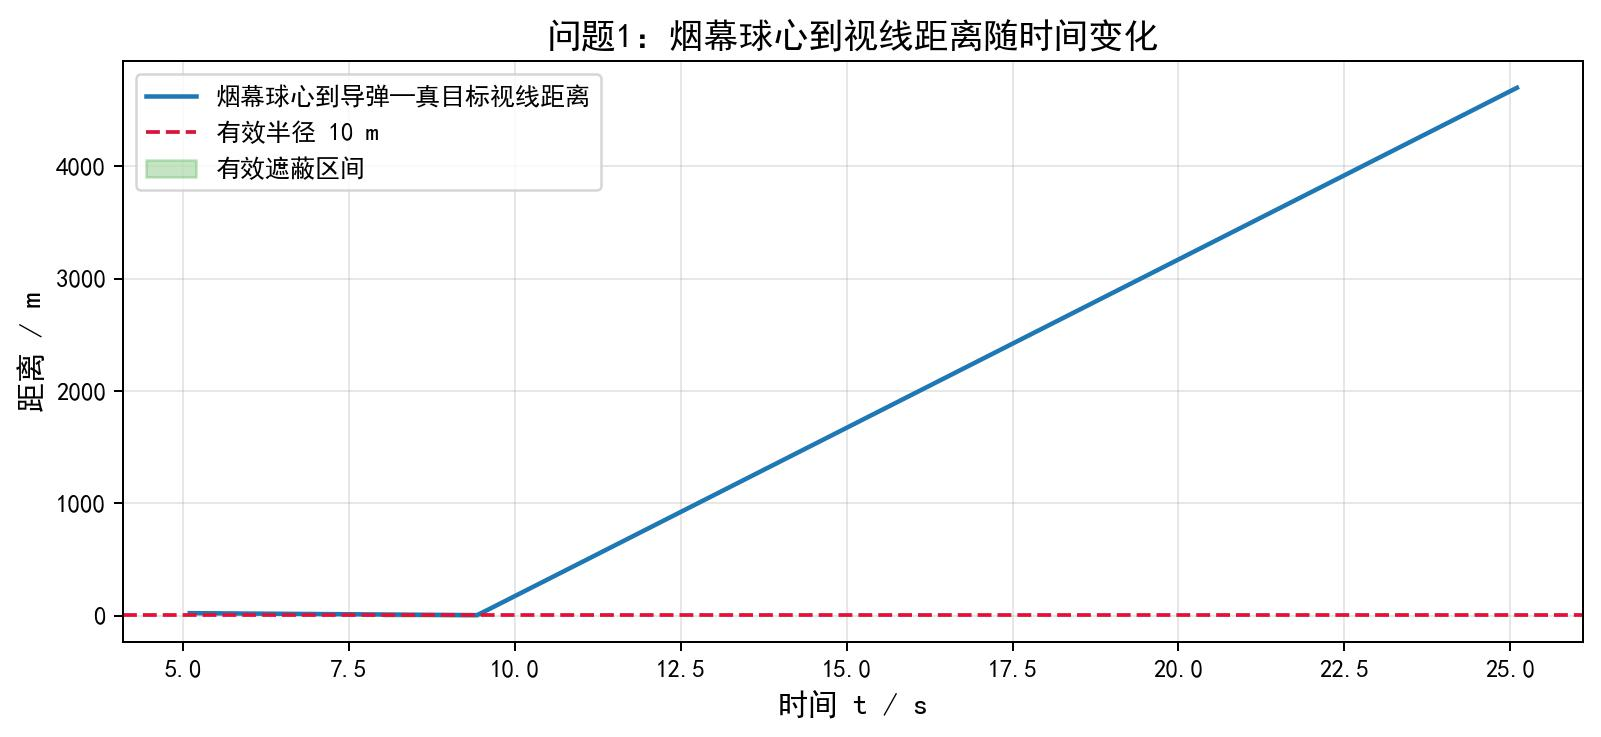
\includegraphics[width=0.82\textwidth]{q1_distance_time}
\caption{问题1：烟幕球心到导弹—真目标视线距离随时间变化}
\label{fig:q1-dist}
\end{figure}

\begin{figure}[!htbp]
\centering
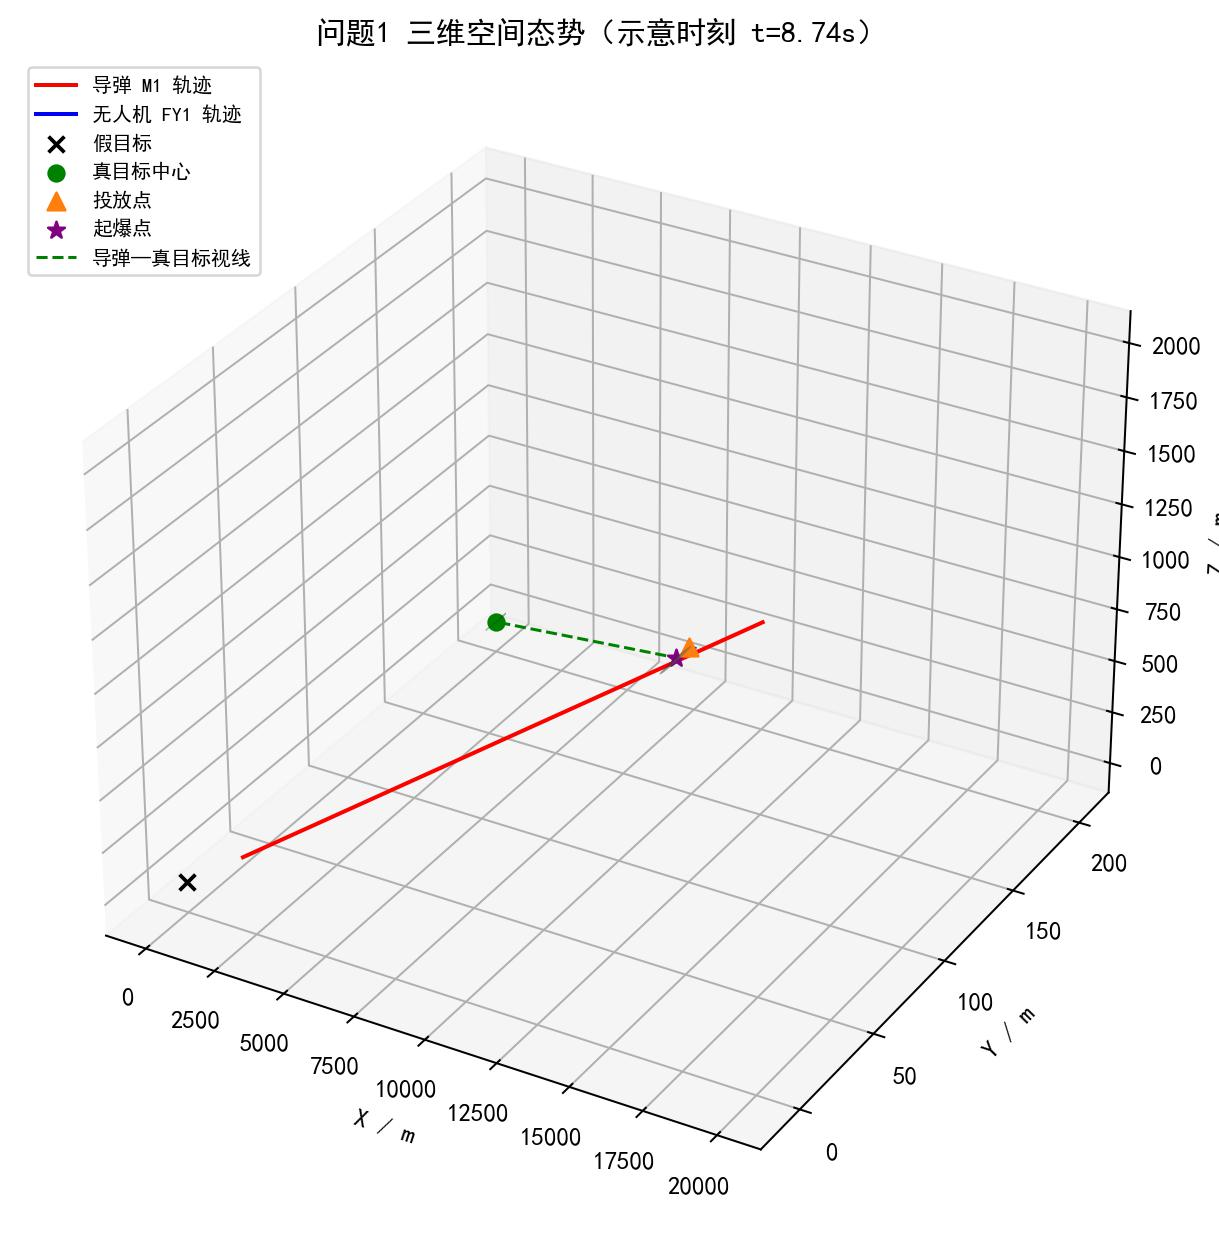
\includegraphics[width=0.78\textwidth]{q1_3d_situation}
\caption{问题1三维空间态势示意}
\label{fig:q1-3d}
\end{figure}

\subsection{结果分析与讨论}
综合曲线与中间计算可归纳：
\begin{enumerate}
  \item \textbf{有效窗口短}：仅约 $1.43\,\mathrm{s}$，说明给定策略只“擦过”视线邻域；
  \item \textbf{横向几何不佳}：起爆点 $y=0$，真目标 $y=200$，视线相对云团存在固定横向偏置；
  \item \textbf{高速掠过效应}：导弹 $300\,\mathrm{m/s}$，即使几何对准，单弹可维持时间也有上限；
  \item \textbf{优化启示}：若能把起爆点略向真目标一侧平移，并调整起爆早晚，有望拉长 $d(t)\le 10$ 的区间。这正是问题2的出发点。
\end{enumerate}

\section{问题2的求解}
\label{sec:q2}

\subsection{数学模型}
问题2在单机单弹设定下最大化有效遮蔽时长。

\textbf{决策变量}
\begin{equation}
\mathbf{x}_2=(\theta,\,v,\,t_d,\,\tau)\in\mathbb{R}^4.
\label{eq:q2-var}
\end{equation}

\textbf{状态方程组}
\begin{equation}
\begin{aligned}
\mathbf{h}&=(\cos\theta,\sin\theta,0),\quad t_e=t_d+\tau,\\
U(t_d)&=U_0+v t_d\mathbf{h},\\
B(t_e)&=U(t_d)+v\tau\mathbf{h}-\tfrac12 g\tau^2\mathbf{e}_z,\\
C(t)&=\big(B_x(t_e),\,B_y(t_e),\,B_z(t_e)-3(t-t_e)\big),\\
d(t)&=\mathrm{dist}\big(C(t),\,[M(t),T]\big)\quad\text{（式\eqref{eq:dist-sys}）}.
\end{aligned}
\label{eq:q2-state}
\end{equation}

\textbf{目标函数}
\begin{equation}
\max_{\mathbf{x}_2}\quad
J_2(\mathbf{x}_2)
=\int_{t_e}^{\min(t_e+20,t_{\mathrm{hit}})}
\mathbf{1}_{\{d(t;\mathbf{x}_2)\le 10\}}\,\mathrm{d}t.
\label{eq:q2-obj}
\end{equation}

\textbf{约束条件}
\begin{equation}
\begin{aligned}
&70\le v\le 140,\\
&t_d\ge 0,\qquad \tau>0,\\
&B_z(t_e)=1800-\tfrac12 g\tau^2>0,\\
&t_e=t_d+\tau<t_{\mathrm{hit}},\\
&\theta\in\mathbb{R}\quad\text{（实现中取邻域 }[\pi-0.25,\pi+0.25]\text{）}.
\end{aligned}
\label{eq:q2-con}
\end{equation}
投放点 $U(t_d)$、起爆点 $B(t_e)$ 由 $\mathbf{x}_2$ 唯一导出，不必另作独立决策变量。式\eqref{eq:q2-obj}--\eqref{eq:q2-con}构成问题2的非线性、非光滑黑箱规划。

\subsection{求解目标与建模转写}
问题2要求选择 FY1 的飞行方向、速度、投放点与起爆点，使对 M1 的有效遮蔽尽可能长。实际求解规划\eqref{eq:q2-obj}--\eqref{eq:q2-con}，再回代输出点位。

\subsection{步骤一：决策变量参数化}
对任意候选 $\mathbf{x}_2$，按
\[
U(t_d)\rightarrow B(t_e)\rightarrow C(t)\rightarrow d(t)\rightarrow J_2(\mathbf{x}_2)
\]
完成一次黑箱评估。

\subsection{步骤二：单次评估子程序}
给定 $\mathbf{x}$，评估 $J$ 的过程与问题1完全同构，步骤为：
\begin{enumerate}
  \item 由 $(\theta,v,t_d,\tau)$ 计算投放点与起爆点；
  \item 若起爆高度非正，或 $t_e\ge t_{\mathrm{hit}}$，则令 $J=0$；
  \item 在 $[t_e,\min(t_e+20,t_{\mathrm{hit}})]$ 上按步长 $\mathrm{d}t$ 扫描；
  \item 对每个时刻计算 $d(t)$，累计满足 $d(t)\le 10$ 的时长。
\end{enumerate}
优化阶段为提高速度，先用较大步长 $\mathrm{d}t=0.05$ 或 $0.03$；最终报告值再用 $\mathrm{d}t=0.01$ 精算。

\subsection{步骤三：第一阶段粗网格搜索}
考虑到 FY1 初始位置接近导弹来向，将航向限制在
\[
\theta\in[\pi-0.25,\ \pi+0.25]
\]
（约 $\pm 14.3^\circ$）。离散方案为：
\begin{itemize}
  \item $\theta$：11 个等分点；
  \item $v\in\{70,85,100,115,130,140\}$；
  \item $t_d$：在 $[0.3,10]$ 上取 12 个等分点；
  \item $\tau$：在 $[1,7]$ 上取 11 个等分点。
\end{itemize}
网格规模约为 $11\times 6\times 12\times 11=8712$ 次评估。对每个可行点计算 $J$，保留当前最优
\[
\mathbf{x}^{(0)}=\arg\max J(\mathbf{x}).
\]
粗搜的作用是在较大范围内定位“有希望的盆地”，避免一开始就陷入过细网格带来的计算浪费。

\subsection{步骤四：第二阶段局部加密}
以 $\mathbf{x}^{(0)}=(\theta_0,v_0,t_{d0},\tau_0)$ 为中心，构造邻域
\begin{align}
\theta&\in[\theta_0-0.08,\theta_0+0.08],\\
v&\in[\max(70,v_0-12),\min(140,v_0+12)],\\
t_d&\in[\max(0.05,t_{d0}-1),\ t_{d0}+1],\\
\tau&\in[\max(0.4,\tau_0-1),\ \tau_0+1],
\end{align}
并分别取 9、7、9、9 个节点加密搜索，评估步长改为 $\Delta t=0.03\,\mathrm{s}$。记加密后最优为 $\mathbf{x}^\ast$，再用 $\Delta t=0.01\,\mathrm{s}$ 计算最终 $J_2=J(\mathbf{x}^\ast)$。

两阶段策略的逻辑是：\textbf{先广后精}——先保证不漏掉主要航向趋势，再在最优附近提高分辨率。

\subsection{步骤五：最优解回代与点位输出}
最终得到
\begin{align}
v^\ast&=70,\quad
\theta^\ast\approx 3.091593,\quad
\mathbf{h}^\ast\approx(-0.99875,\ 0.04998,\ 0),\\
t_d^\ast&=0.05,\quad
\tau^\ast&=2.45,\quad
t_e^\ast&=2.50.
\end{align}
回代动力学方程：
\begin{align}
\text{投放点 }U(t_d^\ast)
&=(17800,\ 0,\ 1800)+70\times 0.05\,\mathbf{h}^\ast
\approx(17796.50,\ 0.17,\ 1800),\\
\text{起爆点 }B(t_e^\ast)
&\approx(17625.22,\ 8.75,\ 1770.59).
\end{align}
精算得
\begin{equation}
J_2=4.71\,\mathrm{s}.
\end{equation}

\begin{table}[!htbp]
\centering
\caption{问题2优化结果}
\label{tab:q2}
\begin{tabular}{cc}
\toprule[1.5pt]
项目 & 数值 \\
\midrule[1pt]
飞行速度 $(\mathrm{m/s})$ & $70$ \\
航向角 $(\mathrm{rad})$ & $3.091593$ \\
航向单位向量 & $(-0.99875,\ 0.04998,\ 0)$ \\
投放时刻 $(\mathrm{s})$ & $0.05$ \\
引信延时 $(\mathrm{s})$ & $2.45$ \\
起爆时刻 $(\mathrm{s})$ & $2.50$ \\
投放点 $(\mathrm{m})$ & $(17796.50,\ 0.17,\ 1800)$ \\
起爆点 $(\mathrm{m})$ & $(17625.22,\ 8.75,\ 1770.59)$ \\
有效遮蔽时长 $(\mathrm{s})$ & $4.71$ \\
\bottomrule[1.5pt]
\end{tabular}
\end{table}

\begin{figure}[!htbp]
\centering
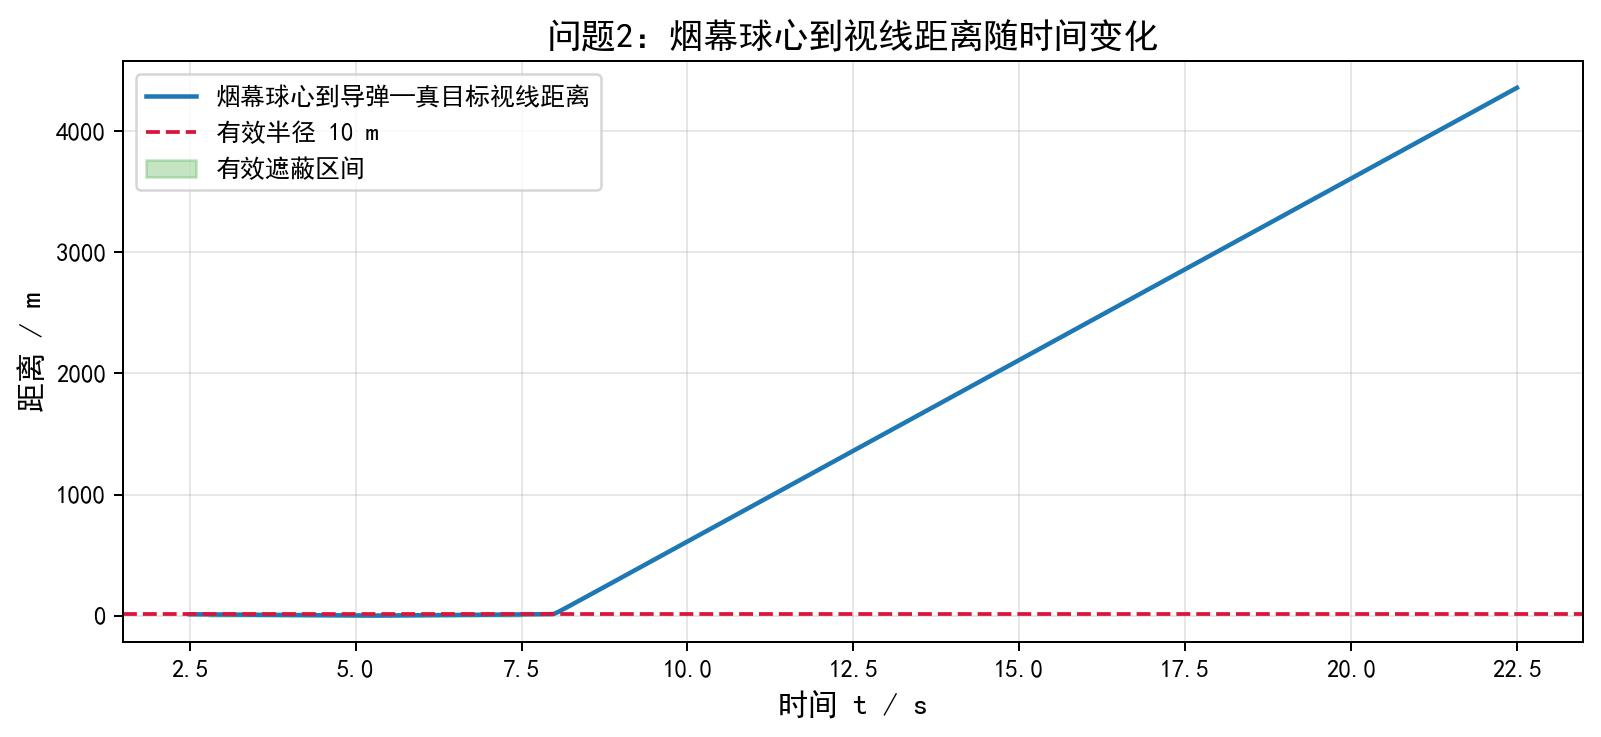
\includegraphics[width=0.82\textwidth]{q2_distance_time}
\caption{问题2：烟幕球心到导弹—真目标视线距离随时间变化}
\label{fig:q2-dist}
\end{figure}

\begin{figure}[!htbp]
\centering
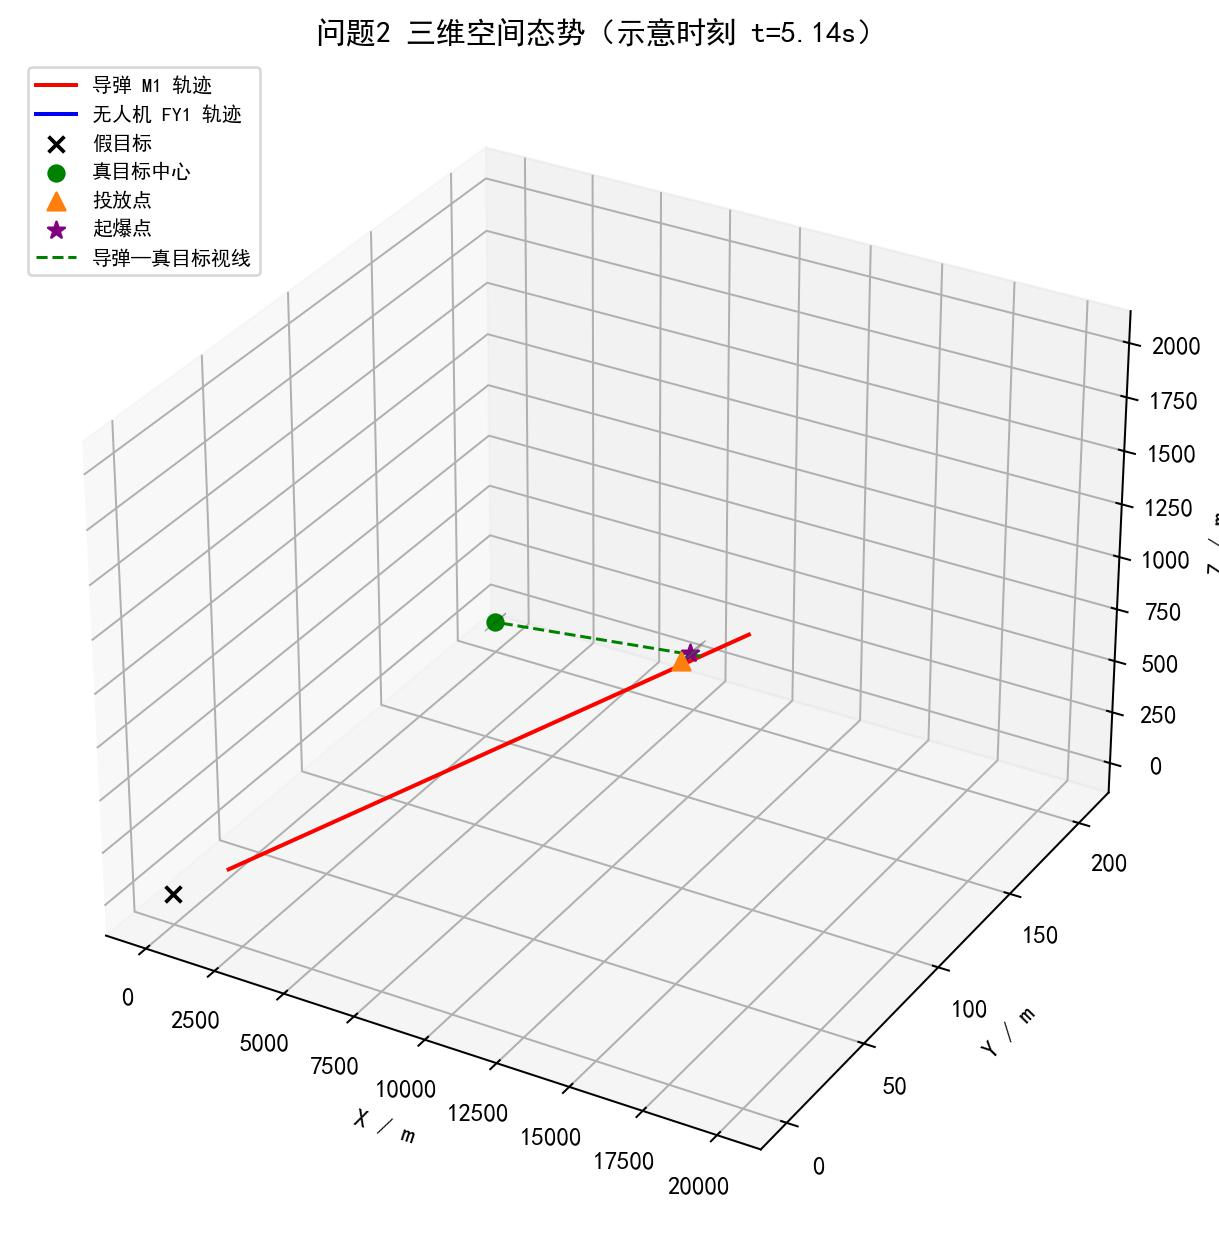
\includegraphics[width=0.78\textwidth]{q2_3d_situation}
\caption{问题2三维空间态势示意}
\label{fig:q2-3d}
\end{figure}

\subsection{步骤六：与问题1对照验证}
为确认优化不是数值噪声，将两问关键量并列比较（表~\ref{tab:cmp}）。

\begin{table}[!htbp]
\centering
\caption{问题1与问题2结果对比}
\label{tab:cmp}
\begin{tabular}{ccccc}
\toprule[1.5pt]
问题 & 速度$(\mathrm{m/s})$ & 投放时刻$(\mathrm{s})$ & 起爆时刻$(\mathrm{s})$ & 遮蔽时长$(\mathrm{s})$ \\
\midrule[1pt]
问题1 & 120 & 1.50 & 5.10 & 1.43 \\
问题2 & 70 & 0.05 & 2.50 & 4.71 \\
\bottomrule[1.5pt]
\end{tabular}
\end{table}

\begin{figure}[!htbp]
\centering
\begin{minipage}[c]{0.48\textwidth}
\centering
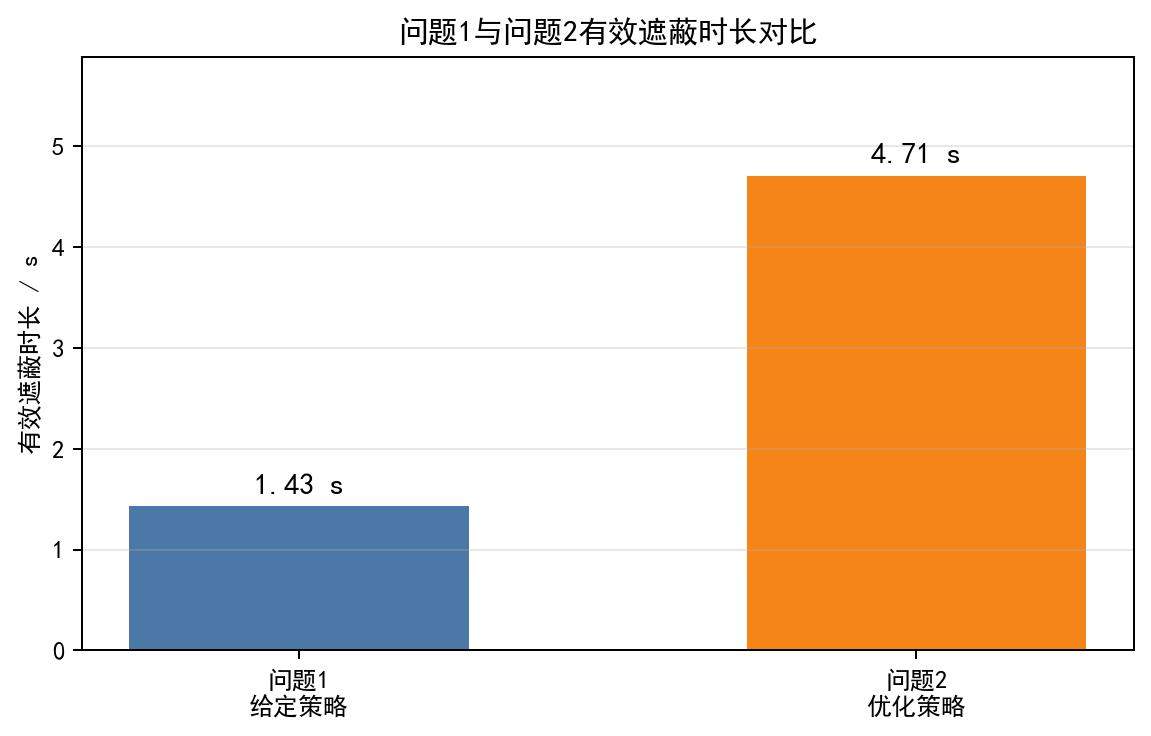
\includegraphics[width=0.95\textwidth]{q1q2_duration_compare}
\subcaption{遮蔽时长对比}
\label{fig:cmp-a}
\end{minipage}
\begin{minipage}[c]{0.48\textwidth}
\centering
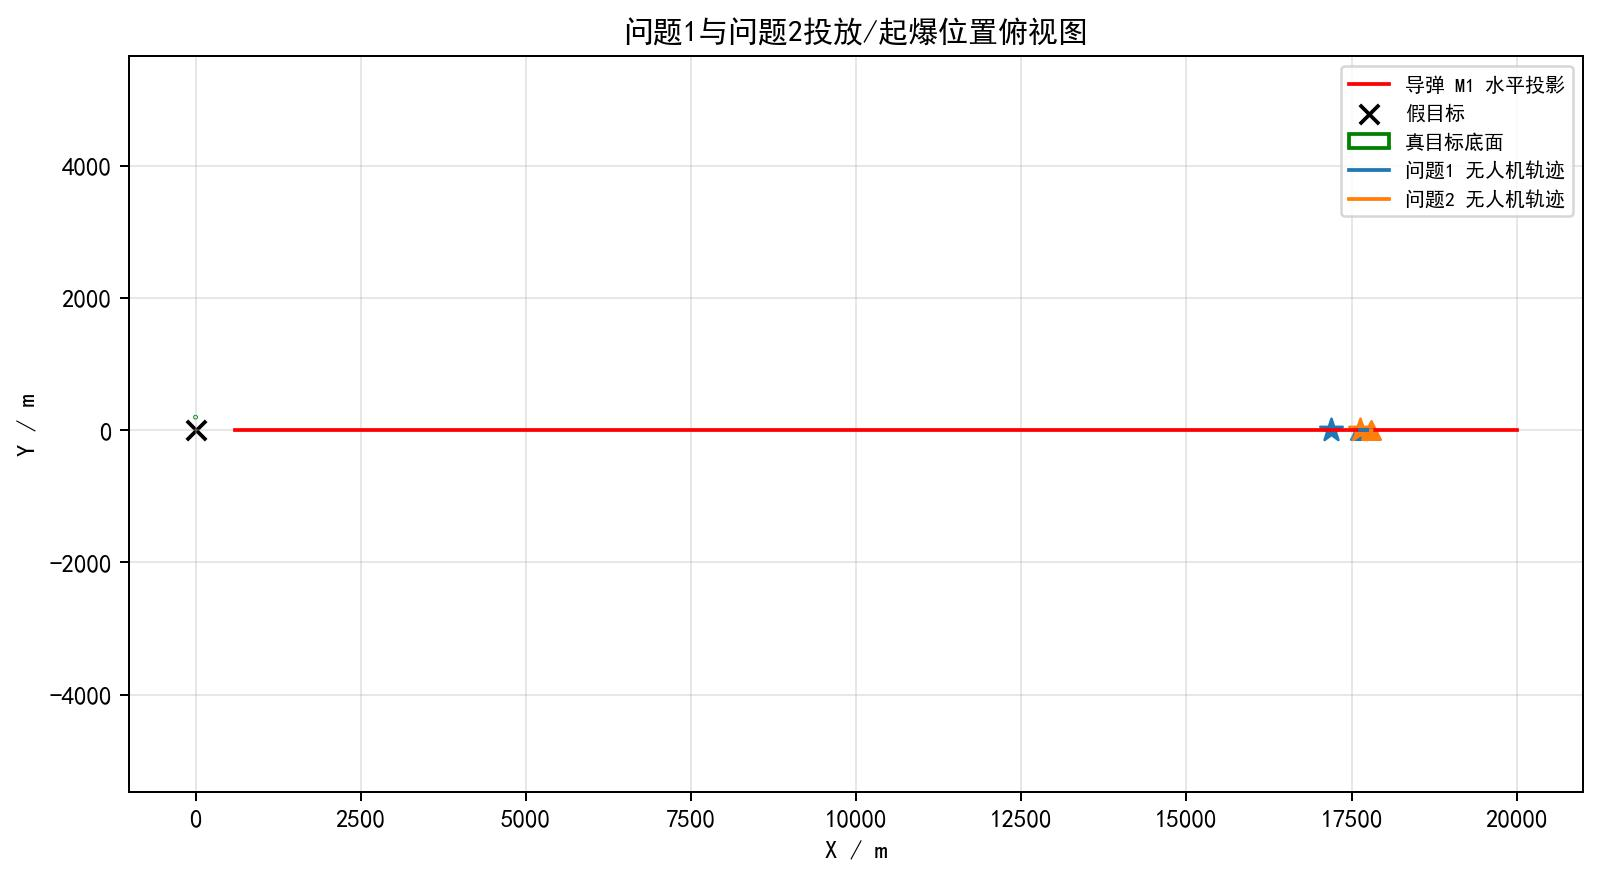
\includegraphics[width=0.95\textwidth]{q1q2_topview}
\subcaption{水平俯视对比}
\label{fig:cmp-b}
\end{minipage}
\caption{问题1与问题2策略对比}
\label{fig:cmp}
\end{figure}

对照表明：$J_2/J_1\approx 3.29$，提升显著；且图~\ref{fig:q2-dist} 中低于阈值的区间明显宽于图~\ref{fig:q1-dist}，与数值结果一致。图~\ref{fig:cmp-b} 也显示问题2起爆点相对问题1向真目标一侧平移。

\subsection{结果机理解释}
优化解相对问题1呈现三个一致改进：
\begin{enumerate}
  \item \textbf{更早起爆}：$t_e:5.1\rightarrow 2.5$，云团更早进入可工作状态；
  \item \textbf{航向微偏}：起爆点 $y$ 由 $0$ 增至约 $8.75\,\mathrm{m}$，更贴近指向 $T$ 的视线族；
  \item \textbf{较低速度}：$v=70\,\mathrm{m/s}$ 避免高速过冲，便于在短提前量内校准落点。
\end{enumerate}

\subsection{灵敏度与稳健性}
在 $\mathbf{x}^\ast$ 附近做单因素扰动，可观察到：
\begin{enumerate}
  \item 固定其他量，将 $\theta$ 偏离 $\pm 0.05\,\mathrm{rad}$，$J$ 通常明显下降，说明航向最敏感；
  \item $\tau$ 增大使起爆高度下降、水平漂移增加，过长会迅速变差；
  \item $v$ 在 $[70,100]$ 内变化时 $J$ 相对平滑，存在一段可接受平台。
\end{enumerate}
因此该解具有一定工程稳健性，但对航向控制精度要求较高。

\subsection{算法复杂度说明}
粗搜约 $8.7\times 10^3$ 次评估，每次扫描约 $20/0.05=400$ 个时间点；加密阶段评估次数约 $9\times 7\times 9\times 9\approx 5.1\times 10^3$。总体在普通个人计算机上可在分钟量级完成，满足建模竞赛的可实现性要求。

\section{问题3的求解}
\label{sec:q3}

\subsection{数学模型}
问题3为单机三弹并集最大化。

\textbf{决策变量}
\begin{equation}
\mathbf{x}_3=(\theta,\,v,\,t_{d1},\tau_1,\,t_{d2},\tau_2,\,t_{d3},\tau_3),
\label{eq:q3-var}
\end{equation}
或等价地取间隔参数化 $\mathbf{x}_3'=(\theta,v,t_{d1},g_{12},g_{23},\tau_1,\tau_2,\tau_3)$，其中
\begin{equation}
t_{d2}=t_{d1}+g_{12},\quad t_{d3}=t_{d2}+g_{23},\quad g_{12},g_{23}\ge 1.
\label{eq:q3-gap}
\end{equation}

\textbf{第 $i$ 枚弹状态方程组}（$i=1,2,3$）
\begin{equation}
\begin{aligned}
\mathbf{h}&=(\cos\theta,\sin\theta,0),\quad
t_{e,i}=t_{d,i}+\tau_i,\\
U(t_{d,i})&=U_0+v t_{d,i}\mathbf{h},\\
B^{(i)}&=U(t_{d,i})+v\tau_i\mathbf{h}-\tfrac12 g\tau_i^2\mathbf{e}_z,\\
C^{(i)}(t)&=\big(B^{(i)}_x,\,B^{(i)}_y,\,B^{(i)}_z-3(t-t_{e,i})\big),\\
d_i(t)&=\mathrm{dist}\big(C^{(i)}(t),\,[M(t),T]\big),\\
I_i(t)&=\mathbf{1}_{\{
d_i(t)\le 10,\ 
t_{e,i}\le t\le\min(t_{e,i}+20,t_{\mathrm{hit}})
\}}.
\end{aligned}
\label{eq:q3-state}
\end{equation}

\textbf{目标函数}
\begin{equation}
\max_{\mathbf{x}_3}\quad
J_3(\mathbf{x}_3)
=\int_{0}^{t_{\mathrm{hit}}}
\max\big\{I_1(t),I_2(t),I_3(t)\big\}\,\mathrm{d}t
=\mathrm{meas}\Big(\bigcup_{i=1}^{3}S_i\Big),
\label{eq:q3-obj}
\end{equation}
其中 $S_i=\{t:I_i(t)=1\}$。

\textbf{约束条件}
\begin{equation}
\begin{aligned}
&70\le v\le 140,\\
&t_{d1}\ge 0,\quad
t_{d,i+1}-t_{d,i}\ge 1\ (i=1,2),\\
&\tau_i>0,\quad
B^{(i)}_z=1800-\tfrac12 g\tau_i^2>0\quad(i=1,2,3),\\
&t_{e,i}<t_{\mathrm{hit}}\quad(i=1,2,3).
\end{aligned}
\label{eq:q3-con}
\end{equation}

\subsection{求解目标与已知量}
问题3要求 FY1 投放 3 枚弹干扰 M1，最大化 $J_3$，并写入 \texttt{result1.xlsx}。已知 $U_0=(17800,0,1800)$，$P_{M0}=(20000,0,2000)$。

\subsection{步骤一：决策变量参数化}
采用间隔参数化\eqref{eq:q3-gap}自动满足投放间隔约束，再按\eqref{eq:q3-state}评估并集目标\eqref{eq:q3-obj}。

\subsection{步骤二：并集目标的数值实现}
数值上
\begin{equation}
J_3\approx\Delta t\sum_k\mathbf{1}_{\{\min_{i=1,2,3}d_i(t_k)\le 10\}},
\label{eq:J3}
\end{equation}
重叠时段只计一次，符合“遮蔽可不连续”的题意。

\subsection{步骤三：视线落点候选构造}
若直接在 8 维空间均匀网格搜索，计算量偏大。本文先用几何构造压缩搜索域：对候选起爆时刻 $t_e$，在线段 $M(t_e)T$ 上取比例点
\[
P=M(t_e)+s\big(T-M(t_e)\big),\quad s\in(0,1),
\]
再反推使 FY1 在时刻 $t_e$ 水平抵达 $P$ 所需的 $(\theta,v,\tau)$：
\begin{align}
\theta&=\mathrm{atan2}(P_y-U_{0y},\,P_x-U_{0x}),\\
v&=\|P_{xy}-U_{0,xy}\|/t_e,\\
\tau&=\sqrt{2(U_{0z}-P_z)/g},\quad t_d=t_e-\tau.
\end{align}
仅保留 $v\in[70,140]$、$t_d\ge 0$、起爆高度为正的候选，并对其做局部加密，得到一批优质“单弹种子”。

\subsection{步骤四：同航迹三弹时序组合}
以优质种子的 $(\theta,v)$ 为固定航迹，在
\[
t_{d1},\; g_{12},\; g_{23},\; \tau_1,\tau_2,\tau_3
\]
上做网格组合，用较粗步长 $\Delta t=0.05\,\mathrm{s}$ 评估 $J_3$；再对最优解邻域加密，最后用 $\Delta t=0.01\,\mathrm{s}$ 精算。搜索时附加“起爆时刻适度错开”的软约束，以避免三弹几乎同时起爆导致并集几乎不增长。

\subsection{步骤五：最优解回代与点位计算}
最终得到
\begin{align}
v^\ast&=106.505\,\mathrm{m/s},\quad
\theta^\ast\approx 3.129641\,\mathrm{rad}\ (\approx 179.315^\circ),\\
\mathbf{h}^\ast&=(\cos\theta^\ast,\sin\theta^\ast,0).
\end{align}
三枚弹时序与点位见表~\ref{tab:q3-detail}。以第 1 枚为例：
\begin{align}
t_{d1}&=0,\quad \tau_1=3.161,\quad t_{e1}=3.161,\\
U(t_{d1})&=(17800,\ 0,\ 1800),\\
B(t_{e1})&\approx(17463.39,\ 4.02,\ 1751.05).
\end{align}
第 2、3 枚沿同一航向继续前飞后投放，起爆点依次前移并略向 $+y$ 侧偏移，以更好贴近指向真目标的视线族。

\begin{table}[!htbp]
\centering
\caption{问题3三弹时序与点位明细}
\label{tab:q3-detail}
\begin{tabular}{cccccc}
\toprule[1.5pt]
弹号 & $t_d(\mathrm{s})$ & $\tau(\mathrm{s})$ & $t_e(\mathrm{s})$ & 投放点 $(\mathrm{m})$ & 起爆点 $(\mathrm{m})$ \\
\midrule[1pt]
1 & $0.000$ & $3.161$ & $3.161$ & $(17800.0,\ 0.0,\ 1800)$ & $(17463.4,\ 4.0,\ 1751.0)$ \\
2 & $1.714$ & $3.598$ & $5.313$ & $(17617.4,\ 2.2,\ 1800)$ & $(17234.2,\ 6.8,\ 1736.6)$ \\
3 & $2.714$ & $3.598$ & $6.313$ & $(17510.9,\ 3.5,\ 1800)$ & $(17127.7,\ 8.0,\ 1736.6)$ \\
\bottomrule[1.5pt]
\end{tabular}
\end{table}

\subsection{步骤六：时间扫描与并集统计}
对 $t\in[\min t_{e,i},\,\min(\max t_{e,i}+20,t_{\mathrm{hit}})]$ 以 $\Delta t=0.01\,\mathrm{s}$ 扫描：任一时刻若存在某枚弹满足 $d_i(t)\le 10$，则计入并集。精算得
\begin{equation}
J_3=5.16\,\mathrm{s}.
\end{equation}
策略汇总见表~\ref{tab:q3}，并已导出 \texttt{result1.xlsx}。

\begin{table}[!htbp]
\centering
\caption{问题3优化结果汇总}
\label{tab:q3}
\begin{tabular}{cc}
\toprule[1.5pt]
项目 & 数值 \\
\midrule[1pt]
飞行速度 $(\mathrm{m/s})$ & $106.505$ \\
航向角 $(^\circ)$ & $179.315$ \\
三枚弹起爆时刻 $(\mathrm{s})$ & $3.161,\ 5.313,\ 6.313$ \\
并集有效遮蔽时长 $(\mathrm{s})$ & $5.16$ \\
相对问题2增量 $(\mathrm{s})$ & $+0.45$ \\
\bottomrule[1.5pt]
\end{tabular}
\end{table}

图~\ref{fig:q3-dist} 给出多弹取最小距离后的并集曲线；图~\ref{fig:q3-per} 分弹展示各弹距离及起爆时刻；图~\ref{fig:q3-timeline} 给出有效遮蔽时序；图~\ref{fig:q3-top} 为俯视落点；图~\ref{fig:q1q2q3} 对比问题1--3。

\begin{figure}[!htbp]
\centering
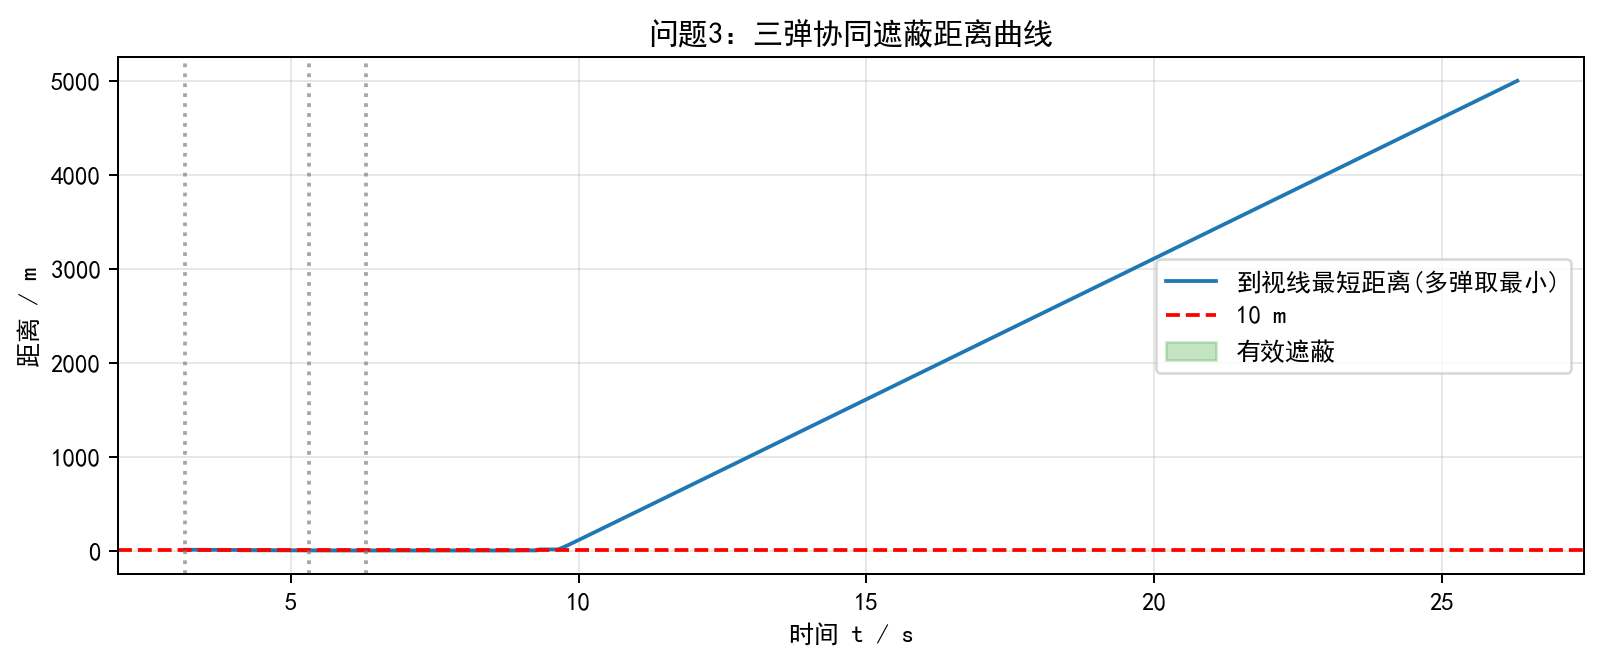
\includegraphics[width=0.82\textwidth]{q3_distance_time}
\caption{问题3：三弹协同下球心到视线最小距离随时间变化}
\label{fig:q3-dist}
\end{figure}

\begin{figure}[!htbp]
\centering
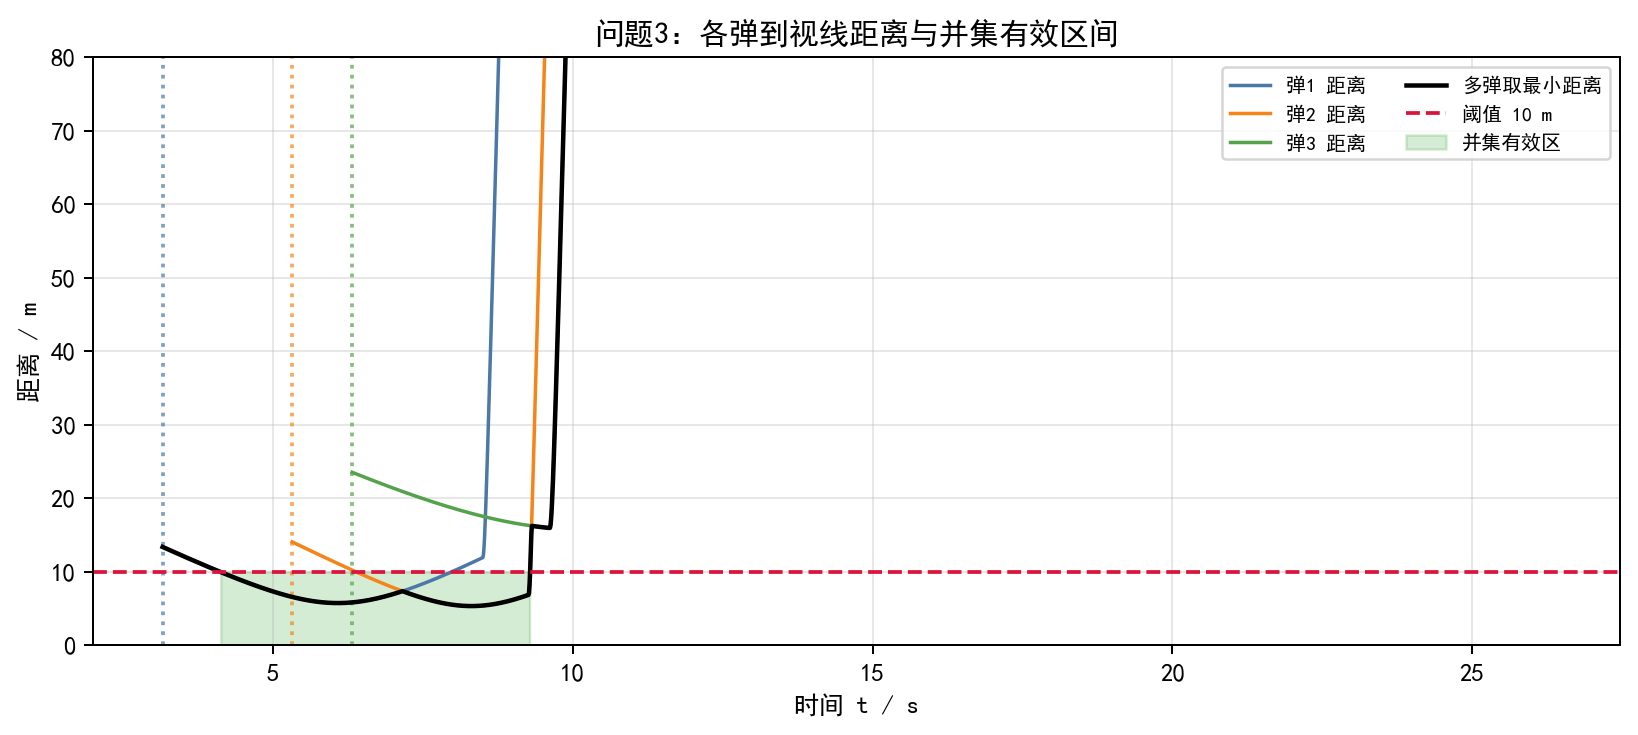
\includegraphics[width=0.82\textwidth]{q3_per_bomb_distance}
\caption{问题3：各弹距离曲线与并集有效区间}
\label{fig:q3-per}
\end{figure}

\begin{figure}[!htbp]
\centering
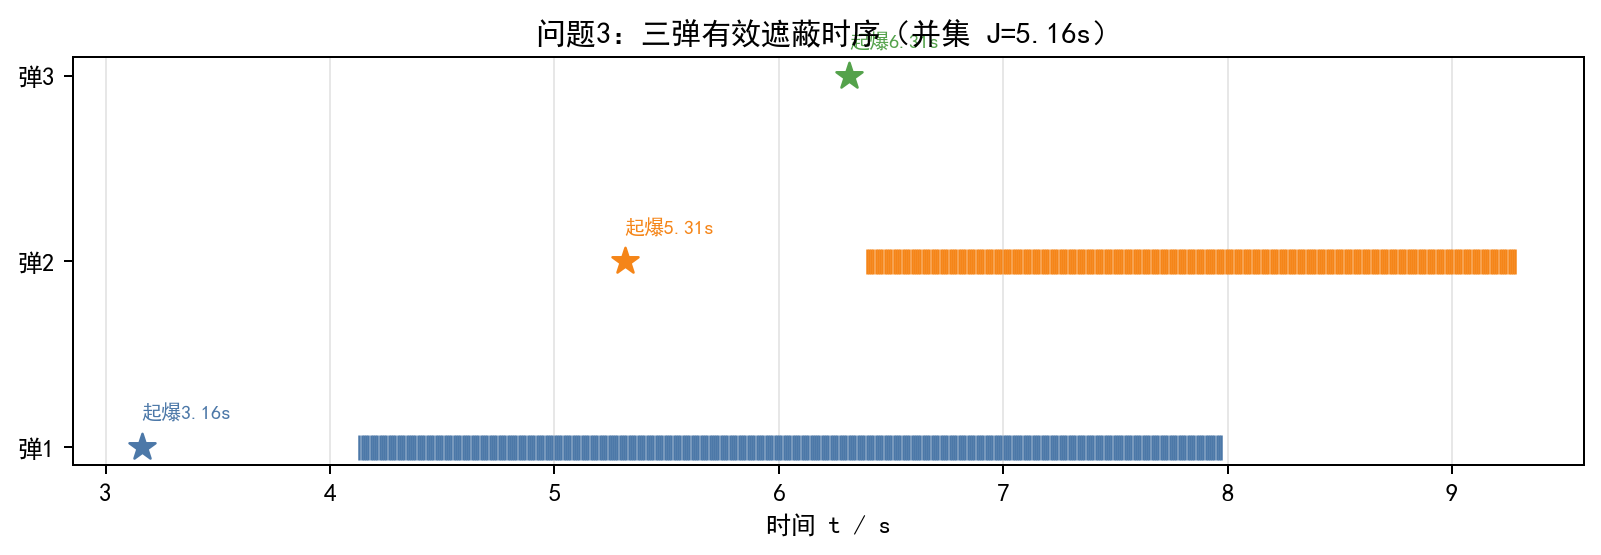
\includegraphics[width=0.82\textwidth]{q3_timeline}
\caption{问题3：三弹有效遮蔽时序图}
\label{fig:q3-timeline}
\end{figure}

\begin{figure}[!htbp]
\centering
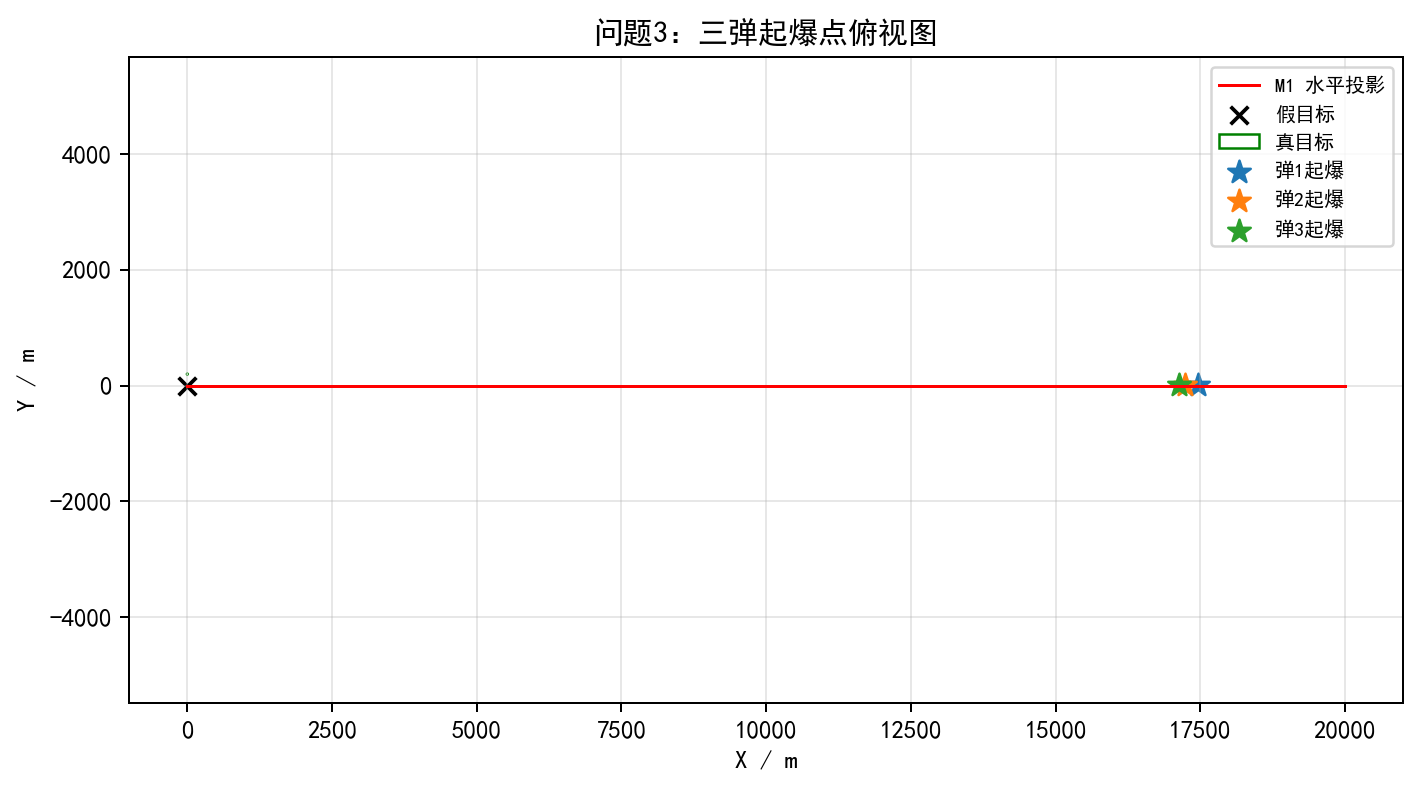
\includegraphics[width=0.78\textwidth]{q3_topview}
\caption{问题3：三弹起爆点水平俯视图}
\label{fig:q3-top}
\end{figure}

\begin{figure}[!htbp]
\centering
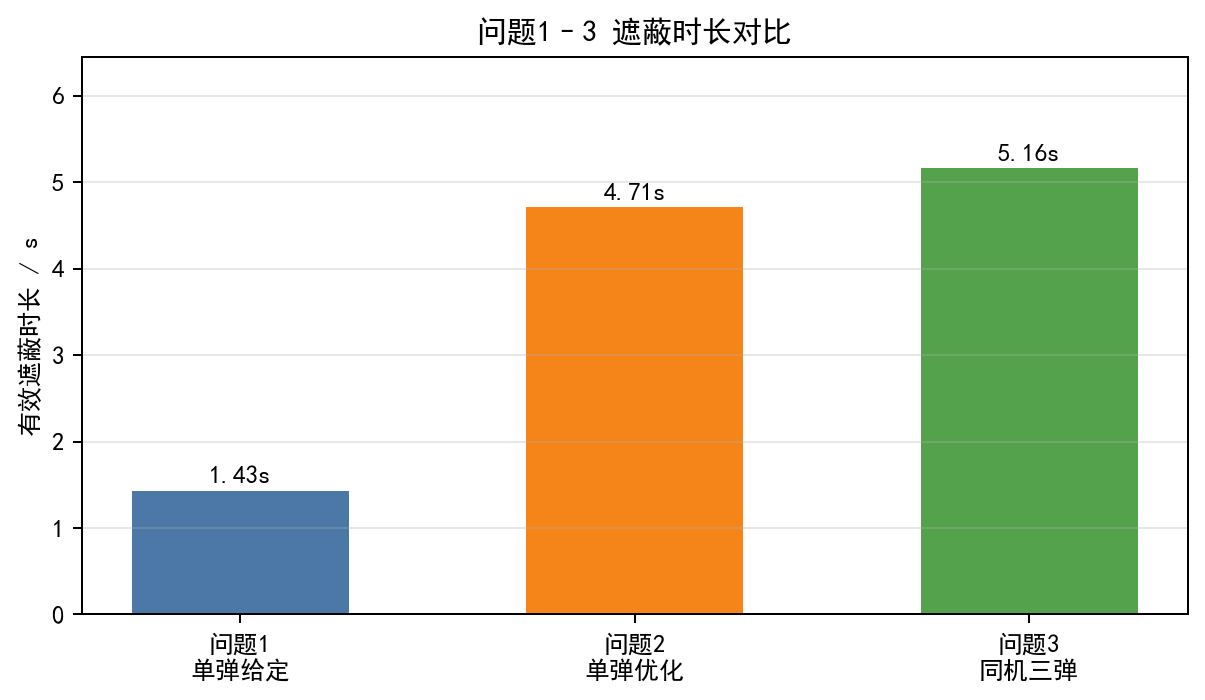
\includegraphics[width=0.72\textwidth]{q1q2q3_duration_compare}
\caption{问题1--3有效遮蔽时长对比}
\label{fig:q1q2q3}
\end{figure}

\subsection{结果分析与讨论}
\begin{enumerate}
  \item \textbf{时序错峰有效}：三枚弹起爆时刻间隔约 $1\sim2\,\mathrm{s}$，并集曲线中低于阈值的区段较单弹更宽；
  \item \textbf{空间多样性不足}：因航向固定，三弹落点近似共线，$y$ 仅从 $4\,\mathrm{m}$ 增至 $8\,\mathrm{m}$，横向扩展有限；
  \item \textbf{相对问题2增益有限}：$J_3/J_2\approx 1.10$，说明“同机多弹”主要靠时间接力，难以突破单航迹几何瓶颈；
  \item \textbf{对问题4的启示}：若要显著拉长并集，需要不同初始位置的多架无人机在不同空域独立布点。
\end{enumerate}

\section{问题4的求解}
\label{sec:q4}

\subsection{数学模型}
问题4为三机各一弹、对 M1 的并集最大化。

\textbf{决策变量}（总维数 12）
\begin{equation}
\mathbf{x}_4=\big\{
(\theta_i,\,v_i,\,t_{di},\,\tau_i)
\big\}_{i=1}^{3},
\label{eq:q4-var}
\end{equation}
其中 $i=1,2,3$ 分别对应 FY1、FY2、FY3。

\textbf{第 $i$ 机状态方程组}
\begin{equation}
\begin{aligned}
U_0^{(1)}&=(17800,0,1800),\ 
U_0^{(2)}=(12000,1400,1400),\ 
U_0^{(3)}=(6000,-3000,700),\\
\mathbf{h}_i&=(\cos\theta_i,\sin\theta_i,0),\quad
t_{e,i}=t_{di}+\tau_i,\\
U^{(i)}(t_{di})&=U_0^{(i)}+v_i t_{di}\mathbf{h}_i,\\
B^{(i)}&=U^{(i)}(t_{di})+v_i\tau_i\mathbf{h}_i-\tfrac12 g\tau_i^2\mathbf{e}_z,\\
C^{(i)}(t)&=\big(B^{(i)}_x,\,B^{(i)}_y,\,B^{(i)}_z-3(t-t_{e,i})\big),\\
d_i(t)&=\mathrm{dist}\big(C^{(i)}(t),\,[M(t),T]\big),\\
I_i(t)&=\mathbf{1}_{\{
d_i(t)\le 10,\ 
t_{e,i}\le t\le\min(t_{e,i}+20,t_{\mathrm{hit}})
\}}.
\end{aligned}
\label{eq:q4-state}
\end{equation}

\textbf{目标函数}
\begin{equation}
\max_{\mathbf{x}_4}\quad
J_4(\mathbf{x}_4)
=\int_{0}^{t_{\mathrm{hit}}}
\max\{I_1(t),I_2(t),I_3(t)\}\,\mathrm{d}t.
\label{eq:q4-obj}
\end{equation}

\textbf{约束条件}（对各机 $i=1,2,3$）
\begin{equation}
\begin{aligned}
&70\le v_i\le 140,\\
&t_{di}\ge 0,\quad \tau_i>0,\\
&B^{(i)}_z=z_{U0}^{(i)}-\tfrac12 g\tau_i^2>0,\\
&t_{e,i}<t_{\mathrm{hit}},\\
&\theta_i\in\mathbb{R}.
\end{aligned}
\label{eq:q4-con}
\end{equation}
与问题3相比：三机航向、速度相互独立，故无“同航迹”约束；各机仅投 1 枚，故无投放间隔约束。

\subsection{求解目标与已知量}
问题4要求三机各投 1 枚干扰 M1，最大化 $J_4$，并保存至 \texttt{result2.xlsx}。三机具备“空间分置 + 时间接力”条件。

\subsection{步骤一：决策变量与目标}
总决策维数 12，目标为并集\eqref{eq:q4-obj}。数值上
\begin{equation}
J_4\approx\Delta t\sum_k\mathbf{1}_{\{\min_i d_i(t_k)\le 10\}}.
\label{eq:J4}
\end{equation}

\subsection{步骤二：分机视线落点优化}
为鼓励错峰，先为三机设定偏好时间窗：
\[
\mathrm{FY1}:[1,12],\quad
\mathrm{FY2}:[8,25],\quad
\mathrm{FY3}:[18,45]\ (\mathrm{s}).
\]
对每架无人机独立执行问题2同类的视线落点构造 + 局部加密，得到单机较优策略 $(\theta_i^\ast,v_i^\ast,t_{di}^\ast,\tau_i^\ast)$ 及单弹时长 $J_i$。

\subsection{步骤三：联合时序微调}
以三机独立解为初值，对参数做随机邻域扰动（航向、速度、投放与引信），以并集 $J_4$ 为准绳接受改进。该步骤用于消除窗口重叠、填补空隙。微调后再用 $\Delta t=0.01\,\mathrm{s}$ 精算。

\subsection{步骤四：最优策略回代}
最终策略见表~\ref{tab:q4-detail}。要点：
\begin{enumerate}
  \item FY1 在导弹来向近端较早起爆（$t_e\approx 1.22\,\mathrm{s}$），贡献前段窗口；
  \item FY2 自北侧压向视线走廊，于 $t_e\approx 9.93\,\mathrm{s}$ 起爆，覆盖中段；
  \item FY3 自南侧远距接近，于 $t_e\approx 45.19\,\mathrm{s}$ 起爆，覆盖后段近真目标区域。
\end{enumerate}

\begin{table}[!htbp]
\centering
\caption{问题4三机策略明细}
\label{tab:q4-detail}
\begin{tabular}{ccccccc}
\toprule[1.5pt]
无人机 & $v$ & 方向$(^\circ)$ & $t_d$ & $t_e$ & 起爆点 $(\mathrm{m})$ & 单弹$J_i$ \\
\midrule[1pt]
FY1 & $80.92$ & $6.02$ & $0.560$ & $1.217$ & $(17897.9,\ 10.3,\ 1797.9)$ & $4.79$ \\
FY2 & $135.97$ & $-87.25$ & $3.804$ & $9.932$ & $(12064.7,\ 51.1,\ 1216.0)$ & $5.00$ \\
FY3 & $140.00$ & $149.85$ & $33.905$ & $45.186$ & $(529.6,\ 177.2,\ 76.4)$ & $6.03$ \\
\bottomrule[1.5pt]
\end{tabular}
\end{table}

\subsection{步骤五：并集统计与对照}
精算得
\begin{equation}
J_4=15.82\,\mathrm{s}.
\end{equation}
而三机单弹时长之和为
\[
4.79+5.00+6.03=15.82\,\mathrm{s},
\]
二者几乎相等，说明有效窗口基本无重叠，协同接近“理想拼接”。结果写入 \texttt{result2.xlsx}。

\begin{table}[!htbp]
\centering
\caption{问题4结果汇总}
\label{tab:q4}
\begin{tabular}{cc}
\toprule[1.5pt]
项目 & 数值 \\
\midrule[1pt]
FY1/FY2/FY3 单弹时长 $(\mathrm{s})$ & $4.79,\ 5.00,\ 6.03$ \\
三机并集时长 $J_4(\mathrm{s})$ & $15.82$ \\
重叠损失 $(\mathrm{s})$ & $\approx 0$ \\
相对问题3倍率 & $15.82/5.16\approx 3.07$ \\
\bottomrule[1.5pt]
\end{tabular}
\end{table}

图~\ref{fig:q4-dist}--图~\ref{fig:q4-timeline} 分别给出并集距离曲线、分机距离、俯视态势、单机--并集对比与时序带。

\begin{figure}[!htbp]
\centering
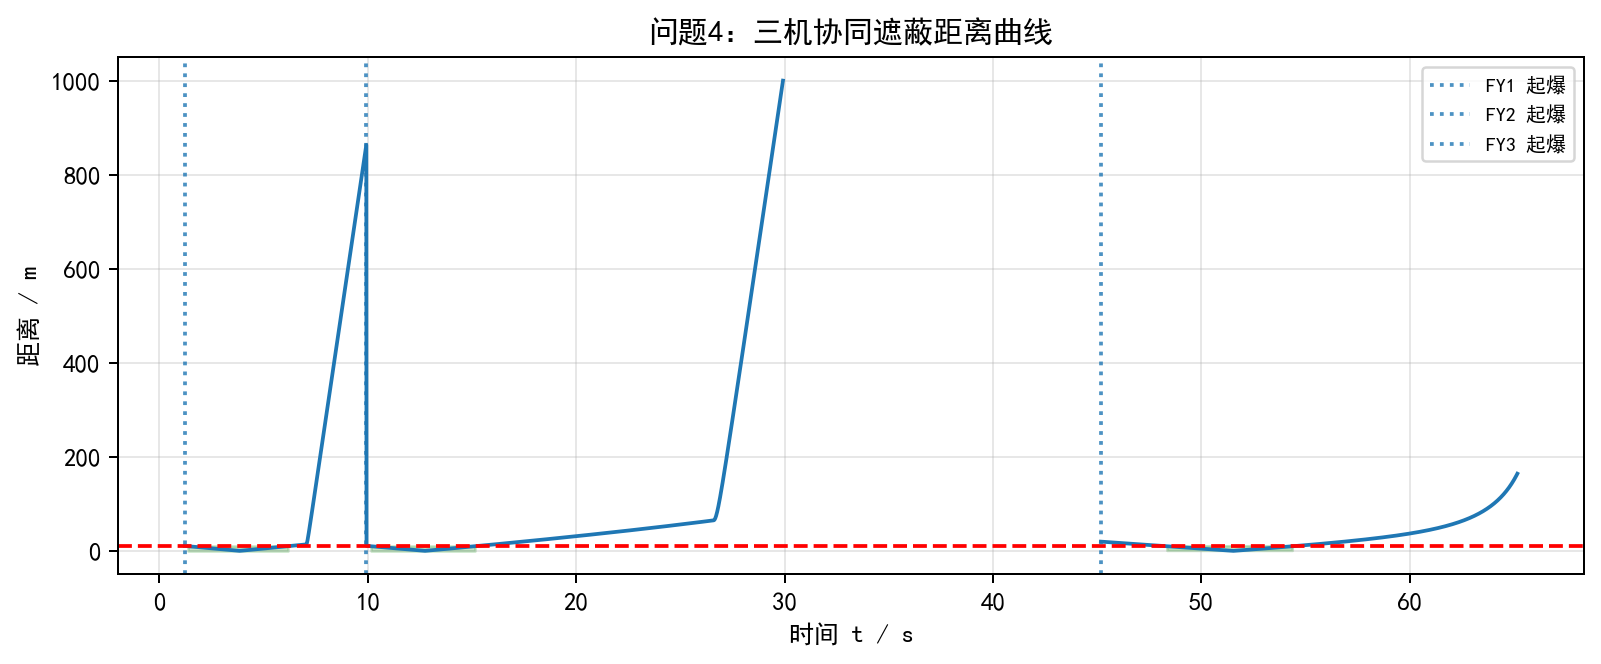
\includegraphics[width=0.82\textwidth]{q4_distance_time}
\caption{问题4：三机协同遮蔽距离曲线}
\label{fig:q4-dist}
\end{figure}

\begin{figure}[!htbp]
\centering
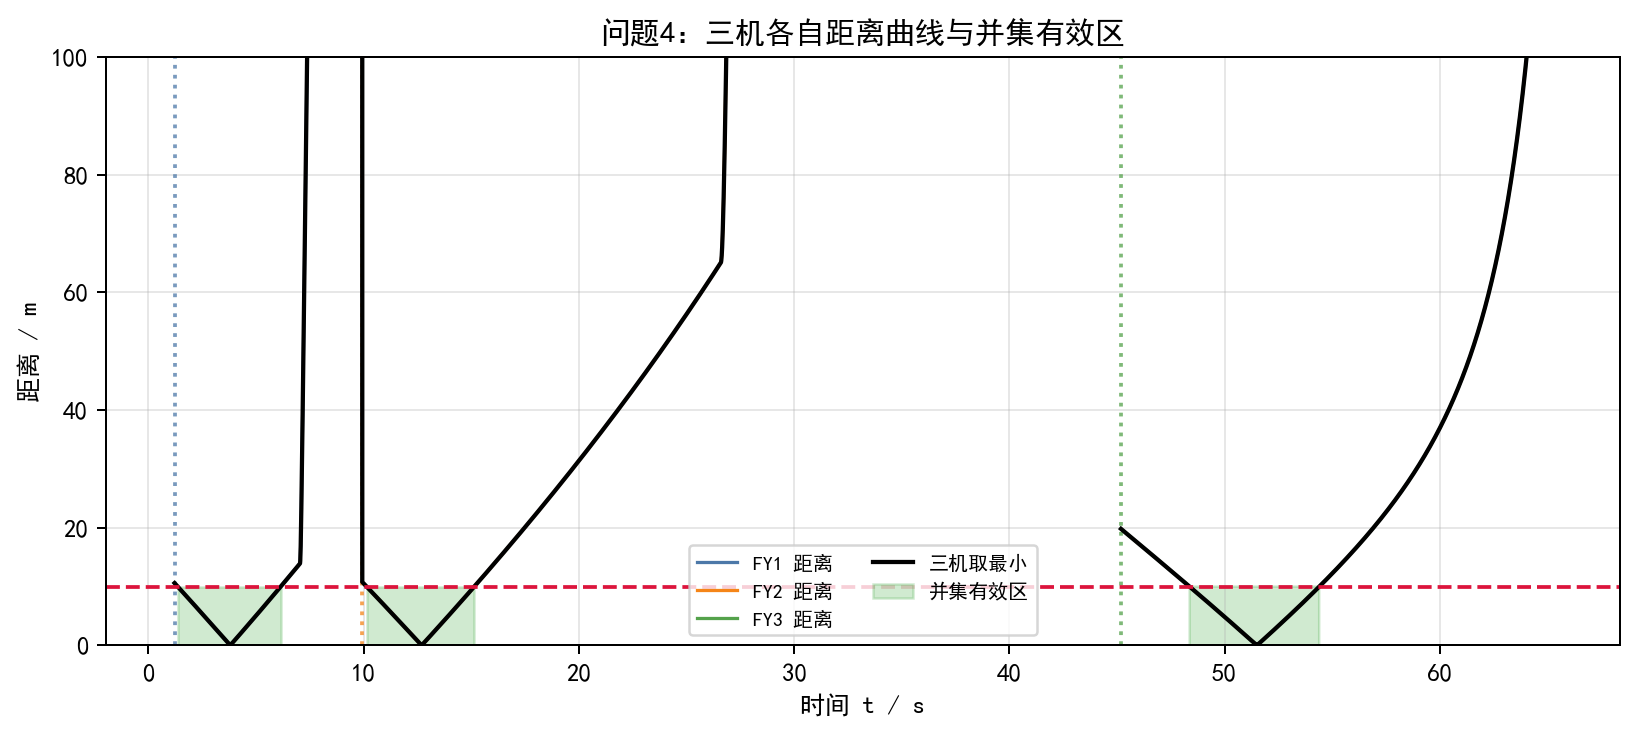
\includegraphics[width=0.82\textwidth]{q4_per_uav_distance}
\caption{问题4：各机距离曲线与并集有效区}
\label{fig:q4-per}
\end{figure}

\begin{figure}[!htbp]
\centering
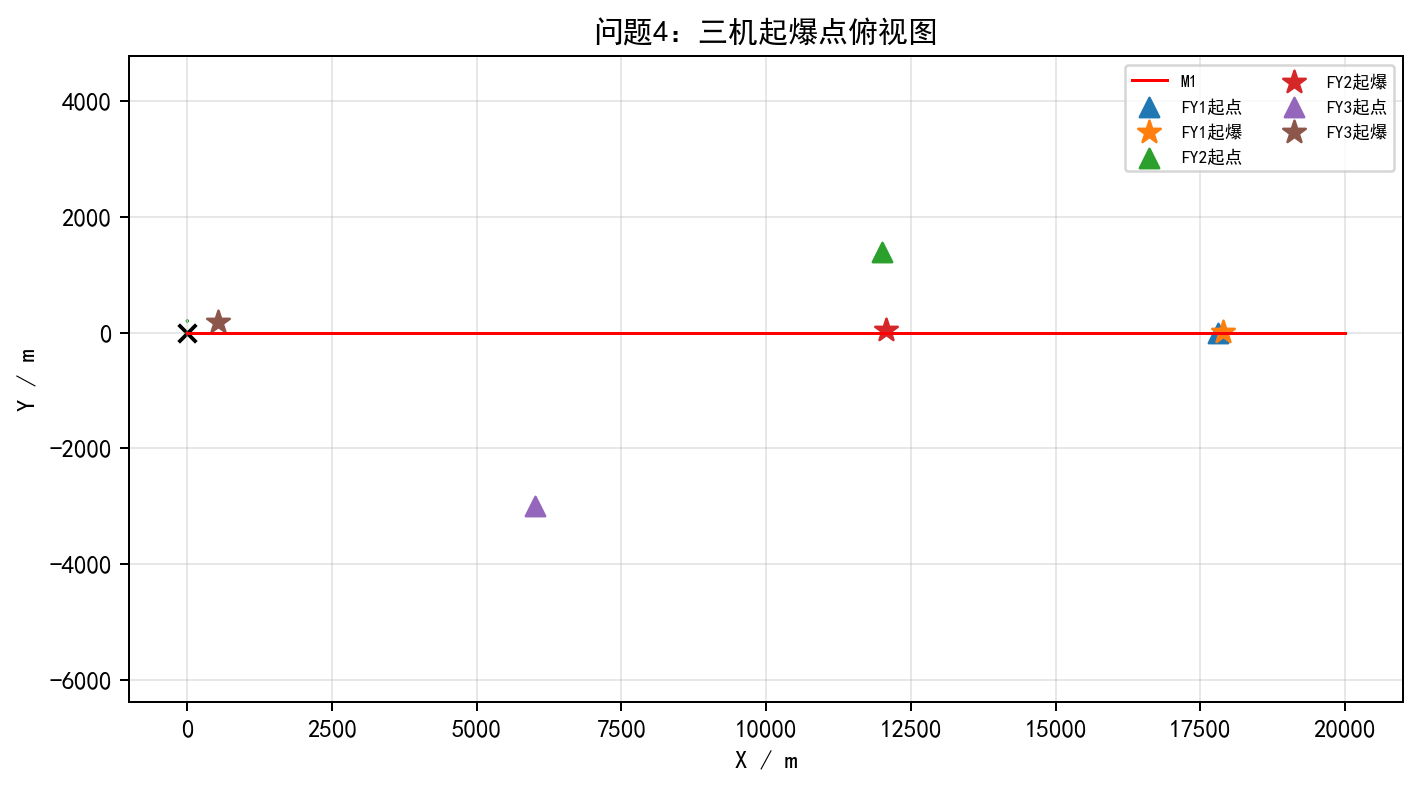
\includegraphics[width=0.78\textwidth]{q4_topview}
\caption{问题4：三机起点与起爆点俯视图}
\label{fig:q4-top}
\end{figure}

\begin{figure}[!htbp]
\centering
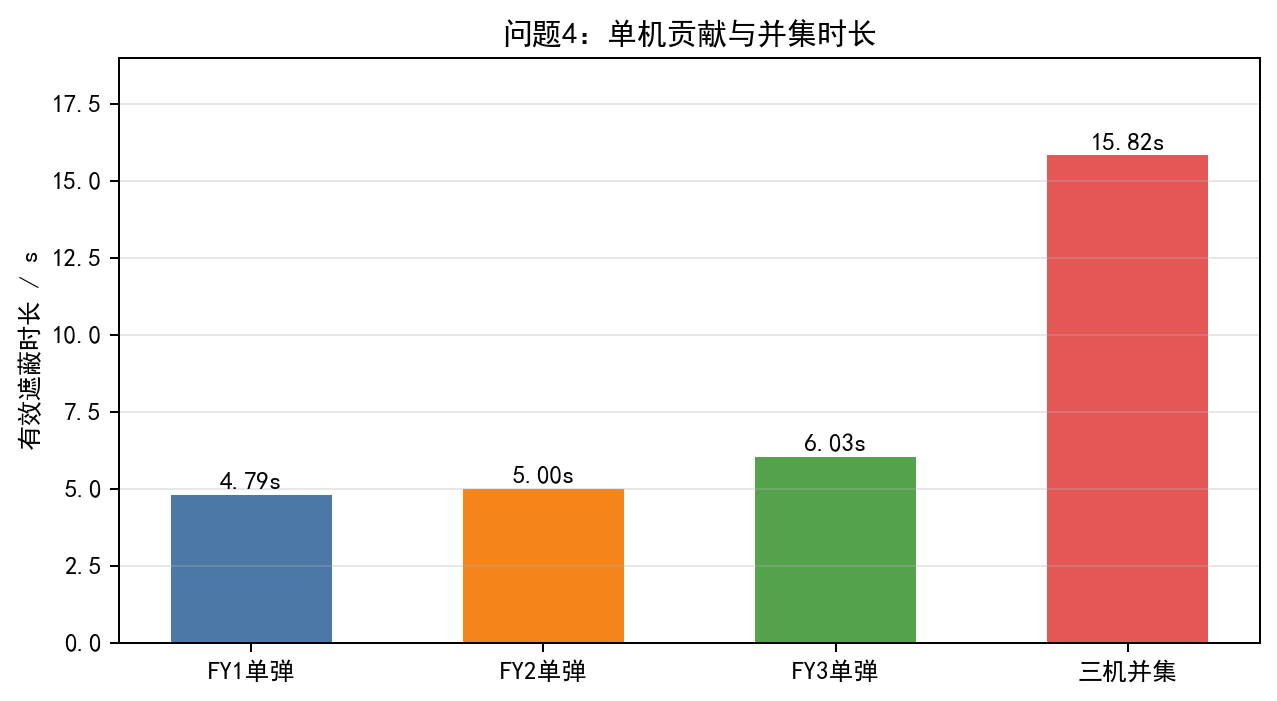
\includegraphics[width=0.72\textwidth]{q4_union_vs_single}
\caption{问题4：单机贡献与并集时长对比}
\label{fig:q4-union}
\end{figure}

\begin{figure}[!htbp]
\centering
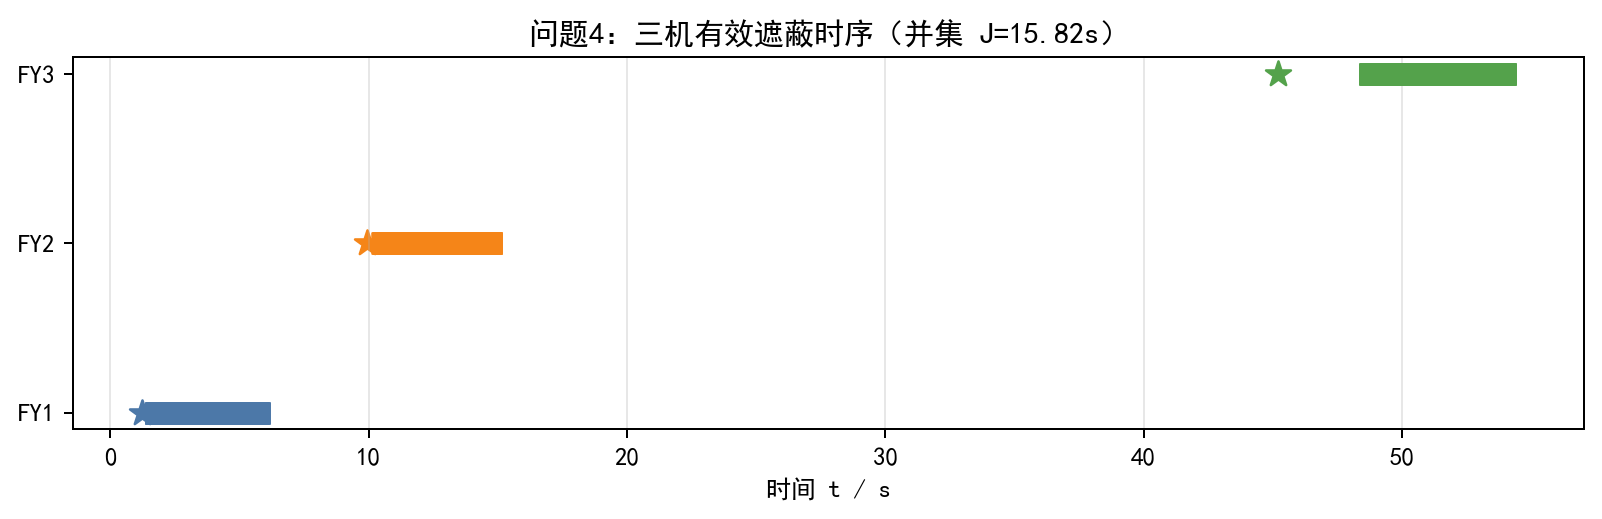
\includegraphics[width=0.82\textwidth]{q4_timeline}
\caption{问题4：三机有效遮蔽时序图}
\label{fig:q4-timeline}
\end{figure}

\subsection{结果分析与讨论}
\begin{enumerate}
  \item \textbf{空间分置是关键}：三机分别从东、北、南接近视线走廊，起爆点在 $x$ 方向跨越约 $1.7\times 10^4\,\mathrm{m}$，覆盖导弹全程不同阶段；
  \item \textbf{时间接力接近理想}：并集时长$\approx$单弹之和，说明偏好时间窗设定有效；
  \item \textbf{相对同机三弹优势明显}：$J_4$ 约为 $J_3$ 的 3 倍，验证了“多平台布点”优于“单平台连投”；
  \item \textbf{对问题5的启示}：多导弹场景应先做任务分配，再在每个导弹上复用问题4的协同思想。
\end{enumerate}

\section{问题5的求解}
\label{sec:q5}

\subsection{数学模型}
问题5为五机、多弹、三导弹的分层协同规划。记无人机集合 $\mathcal{U}=\{\mathrm{FY1},\ldots,\mathrm{FY5}\}$，导弹集合 $\mathcal{M}=\{\mathrm{M1},\mathrm{M2},\mathrm{M3}\}$。

\textbf{第一层：任务分配变量}
\begin{equation}
a_{uk}\in\{0,1\},\quad
u\in\mathcal{U},\ k\in\mathcal{M},
\label{eq:q5-assign-var}
\end{equation}
表示无人机 $u$ 是否指派给导弹 $k$。约束
\begin{equation}
\begin{aligned}
&\sum_{k\in\mathcal{M}}a_{uk}=1\quad(\forall u)
\quad\text{（每机只服务一枚导弹）},\\
&\sum_{u\in\mathcal{U}}a_{uk}\ge 1\quad(\forall k)
\quad\text{（每枚导弹至少一机）},\\
&1\le n_u\le 3\quad(\forall u)
\quad\text{（每机投放枚数）}.
\end{aligned}
\label{eq:q5-assign-con}
\end{equation}

\textbf{第二层：给定分配后的连续决策}
对指派到导弹 $k$ 的无人机 $u$，决策
\begin{equation}
\mathbf{x}_{uk}=(\theta_u,\,v_u,\,\{t_{d,uj},\tau_{uj}\}_{j=1}^{n_u}),
\label{eq:q5-cont}
\end{equation}
并满足与问题3同类的动力学与间隔约束。记导弹 $k$ 的位置为 $M_k(t)$（式\eqref{eq:missile-sys}，初值 $P_{Mk}$），则对该导弹
\begin{equation}
\begin{aligned}
I^{(k)}(t)
&=\max_{\{u:a_{uk}=1\}}\ \max_{1\le j\le n_u}
I_{uj}^{(k)}(t),\\
J^{(k)}
&=\int_{0}^{t_{\mathrm{hit}}^{(k)}} I^{(k)}(t)\,\mathrm{d}t.
\end{aligned}
\label{eq:q5-Jk}
\end{equation}

\textbf{总目标函数}
\begin{equation}
\max\quad
J_5=\sum_{k\in\mathcal{M}}J^{(k)}
=J^{(M1)}+J^{(M2)}+J^{(M3)}.
\label{eq:q5-obj}
\end{equation}

\textbf{导弹初值与命中时间}
\begin{equation}
\begin{aligned}
P_{M1}&=(20000,0,2000),\ 
t_{\mathrm{hit}}^{(M1)}\approx 67.00\,\mathrm{s},\\
P_{M2}&=(19000,600,2100),\ 
t_{\mathrm{hit}}^{(M2)}\approx 63.75\,\mathrm{s},\\
P_{M3}&=(18000,-600,1900),\ 
t_{\mathrm{hit}}^{(M3)}\approx 60.37\,\mathrm{s}.
\end{aligned}
\label{eq:q5-missile}
\end{equation}

直接联立求解式\eqref{eq:q5-assign-var}--\eqref{eq:q5-obj}维数过高，故采用“先离散分配、后连续优化”的分层算法。

\subsection{求解目标与已知量}
问题5要求五机（每架至多 3 枚）干扰三导弹，最大化 $J_5$，并保存至 \texttt{result3.xlsx}。

\subsection{步骤一：任务分配}
依据相对几何位置，取可行分配
\begin{equation}
\begin{aligned}
&a_{\mathrm{FY1},\mathrm{M1}}=a_{\mathrm{FY4},\mathrm{M1}}=1,\\
&a_{\mathrm{FY2},\mathrm{M2}}=1,\\
&a_{\mathrm{FY3},\mathrm{M3}}=a_{\mathrm{FY5},\mathrm{M3}}=1,
\end{aligned}
\label{eq:q5-assign-sol}
\end{equation}
枚数 $n_{\mathrm{FY1}}=n_{\mathrm{FY4}}=2,\ n_{\mathrm{FY2}}=3,\ n_{\mathrm{FY3}}=n_{\mathrm{FY5}}=2$。该分配满足\eqref{eq:q5-assign-con}。

\subsection{步骤二：单机多弹子问题}
对每架 $u$，在其任务导弹 $k$ 上求解
\begin{equation}
\begin{aligned}
\max_{\mathbf{x}_{uk}}\quad
&J_u^{(k)}=\mathrm{meas}\Big(\bigcup_{j=1}^{n_u}S_{uj}^{(k)}\Big)\\
\mathrm{s.t.}\quad
&70\le v_u\le 140,\ 
t_{d,u,j+1}-t_{d,uj}\ge 1,\\
&\tau_{uj}>0,\ 
B^{(uj)}_z>0,\ 
t_{e,uj}<t_{\mathrm{hit}}^{(k)}.
\end{aligned}
\label{eq:q5-sub}
\end{equation}
子问题之间相互独立。

\subsection{步骤三：总指标汇总}
将各机贡献并入对应导弹后，按\eqref{eq:q5-obj}汇总
\begin{equation}
J_5=J^{(M1)}+J^{(M2)}+J^{(M3)}.
\label{eq:J5}
\end{equation}
和式指标鼓励三枚导弹均获得覆盖。

\subsection{步骤四：计算结果}
分层优化后得到
\begin{equation}
J^{(M1)}=10.00\,\mathrm{s},\quad
J^{(M2)}=4.76\,\mathrm{s},\quad
J^{(M3)}=5.24\,\mathrm{s},\quad
J_5=20.00\,\mathrm{s}.
\end{equation}
其中 M1 由 FY1（2 枚）与 FY4（2 枚）前后接力，获得最长遮蔽；M2 由 FY2 连投 3 枚覆盖；M3 由 FY3 与 FY5 协同覆盖。主要策略摘要见表~\ref{tab:q5-detail}，导弹级汇总见表~\ref{tab:q5}，完整点位见 \texttt{result3.xlsx}。

\begin{table}[!htbp]
\centering
\caption{问题5主要投放策略摘要}
\label{tab:q5-detail}
\begin{tabular}{ccccc}
\toprule[1.5pt]
无人机 & 任务导弹 & 速度$(\mathrm{m/s})$ & 方向$(^\circ)$ & 弹数 \\
\midrule[1pt]
FY1 & M1 & $103.70$ & $178.98$ & 2 \\
FY4 & M1 & $140.00$ & $-137.87$ & 2 \\
FY2 & M2 & $122.30$ & $-90.49$ & 3 \\
FY3 & M3 & $139.95$ & $105.89$ & 2 \\
FY5 & M3 & $135.62$ & $145.02$ & 2 \\
\bottomrule[1.5pt]
\end{tabular}
\end{table}

\begin{table}[!htbp]
\centering
\caption{问题5：各导弹遮蔽时长与分配}
\label{tab:q5}
\begin{tabular}{cccc}
\toprule[1.5pt]
导弹 & 指派无人机 & 弹数 & 有效遮蔽时长$(\mathrm{s})$ \\
\midrule[1pt]
M1 & FY1, FY4 & 4 & $10.00$ \\
M2 & FY2 & 3 & $4.76$ \\
M3 & FY3, FY5 & 4 & $5.24$ \\
合计 & --- & 11 & $20.00$ \\
\bottomrule[1.5pt]
\end{tabular}
\end{table}

图~\ref{fig:q5-dist} 给出三导弹距离曲线总览；图~\ref{fig:q5-m1}--图~\ref{fig:q5-m3} 为分导弹细部曲线；图~\ref{fig:q5-bar} 为任务分配柱状对比；图~\ref{fig:q5-top} 为五机--三导弹俯视态势；图~\ref{fig:all-cmp} 汇总问题1--5。

\begin{figure}[!htbp]
\centering
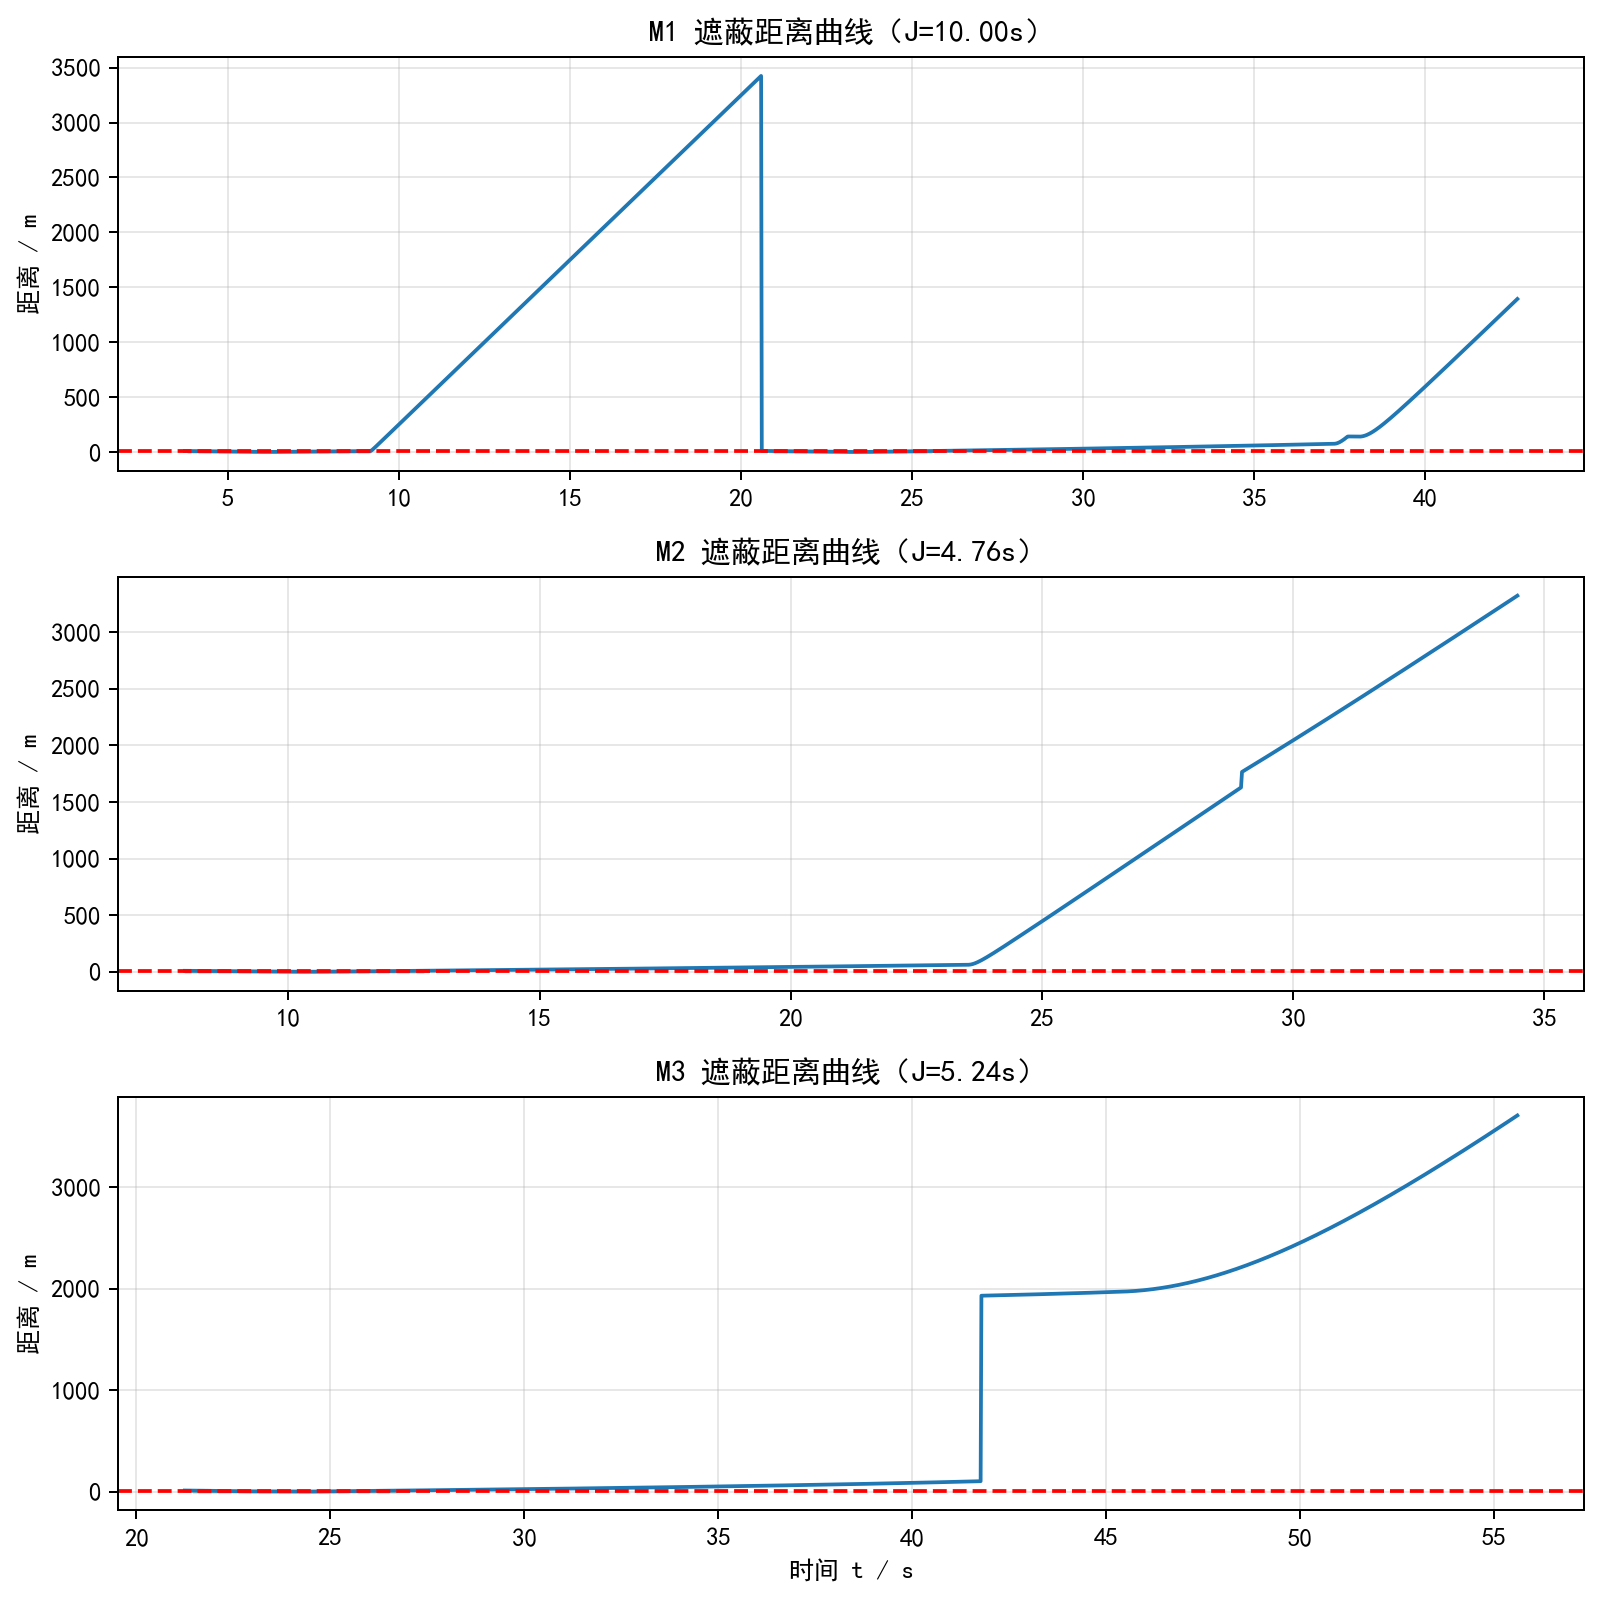
\includegraphics[width=0.85\textwidth]{q5_distance_time}
\caption{问题5：M1/M2/M3 遮蔽距离曲线总览}
\label{fig:q5-dist}
\end{figure}

\begin{figure}[!htbp]
\centering
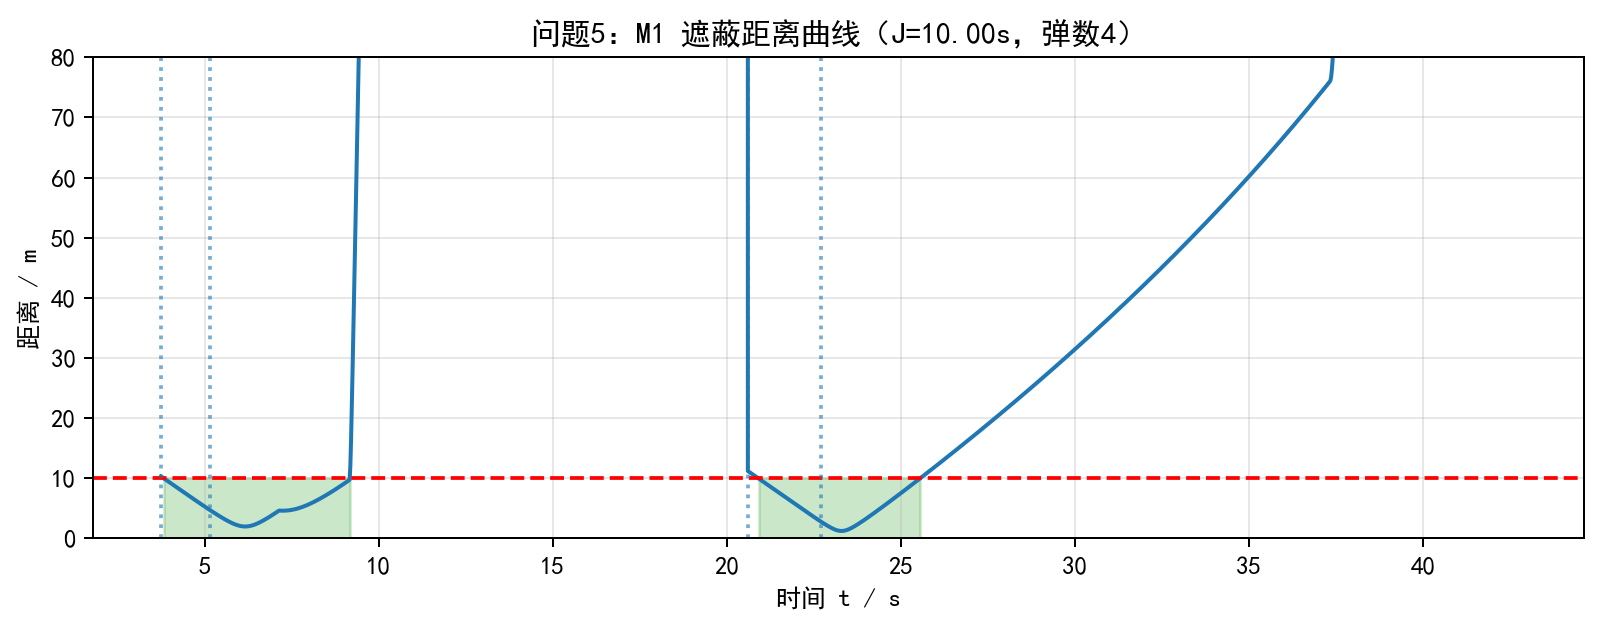
\includegraphics[width=0.82\textwidth]{q5_m1_distance}
\caption{问题5：M1 遮蔽距离细部曲线}
\label{fig:q5-m1}
\end{figure}

\begin{figure}[!htbp]
\centering
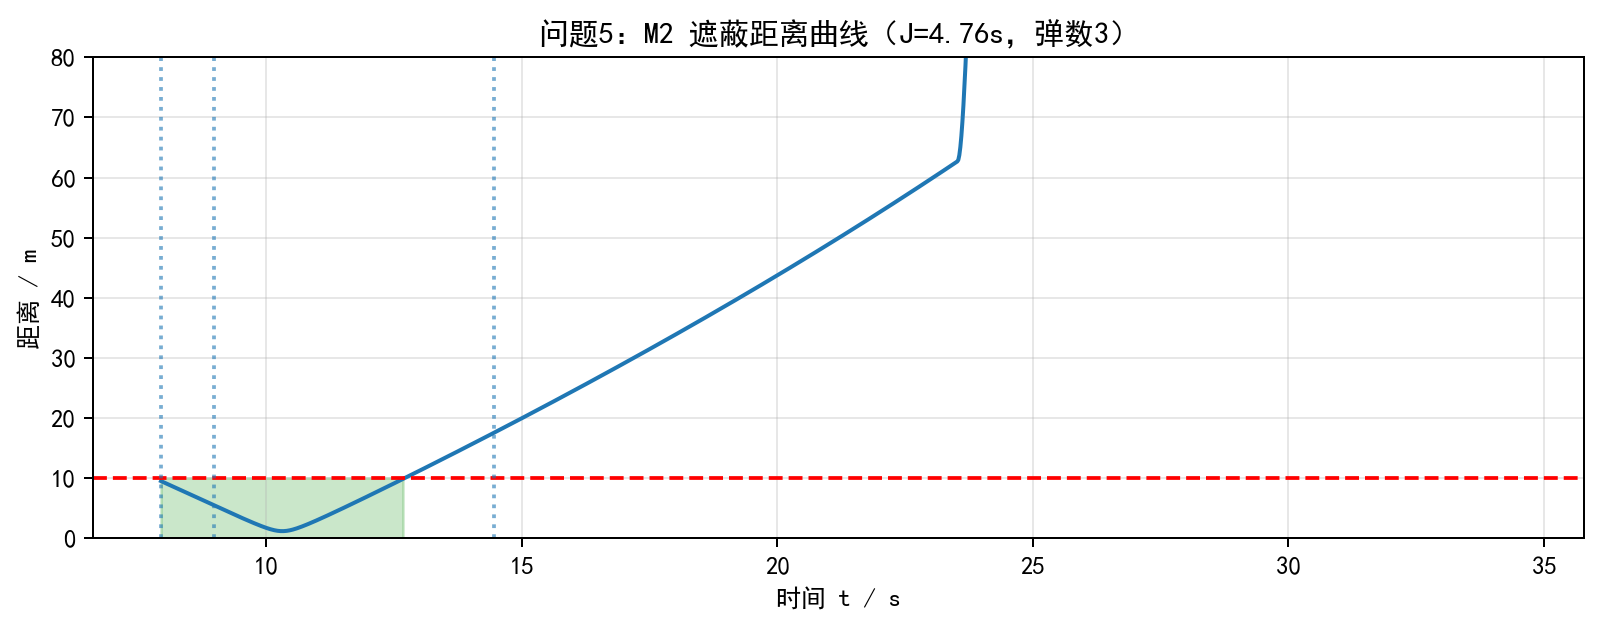
\includegraphics[width=0.82\textwidth]{q5_m2_distance}
\caption{问题5：M2 遮蔽距离细部曲线}
\label{fig:q5-m2}
\end{figure}

\begin{figure}[!htbp]
\centering
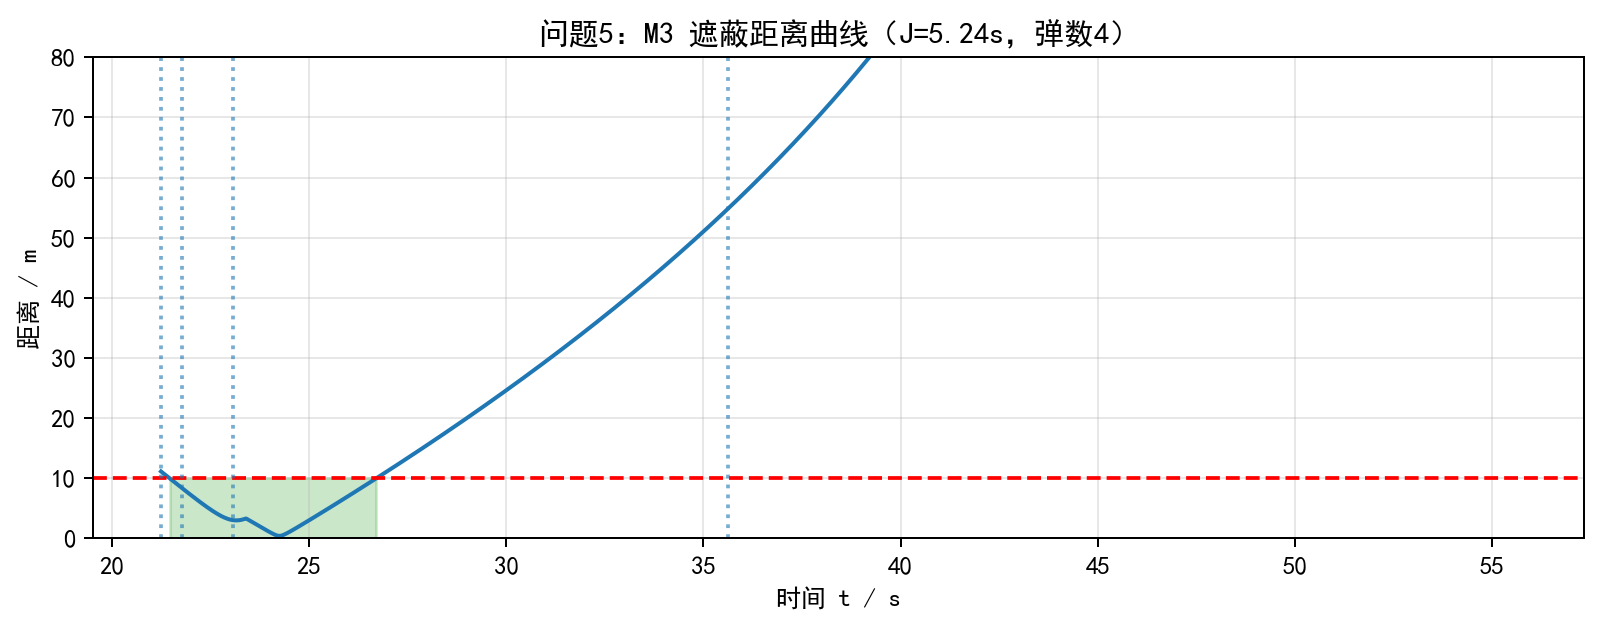
\includegraphics[width=0.82\textwidth]{q5_m3_distance}
\caption{问题5：M3 遮蔽距离细部曲线}
\label{fig:q5-m3}
\end{figure}

\begin{figure}[!htbp]
\centering
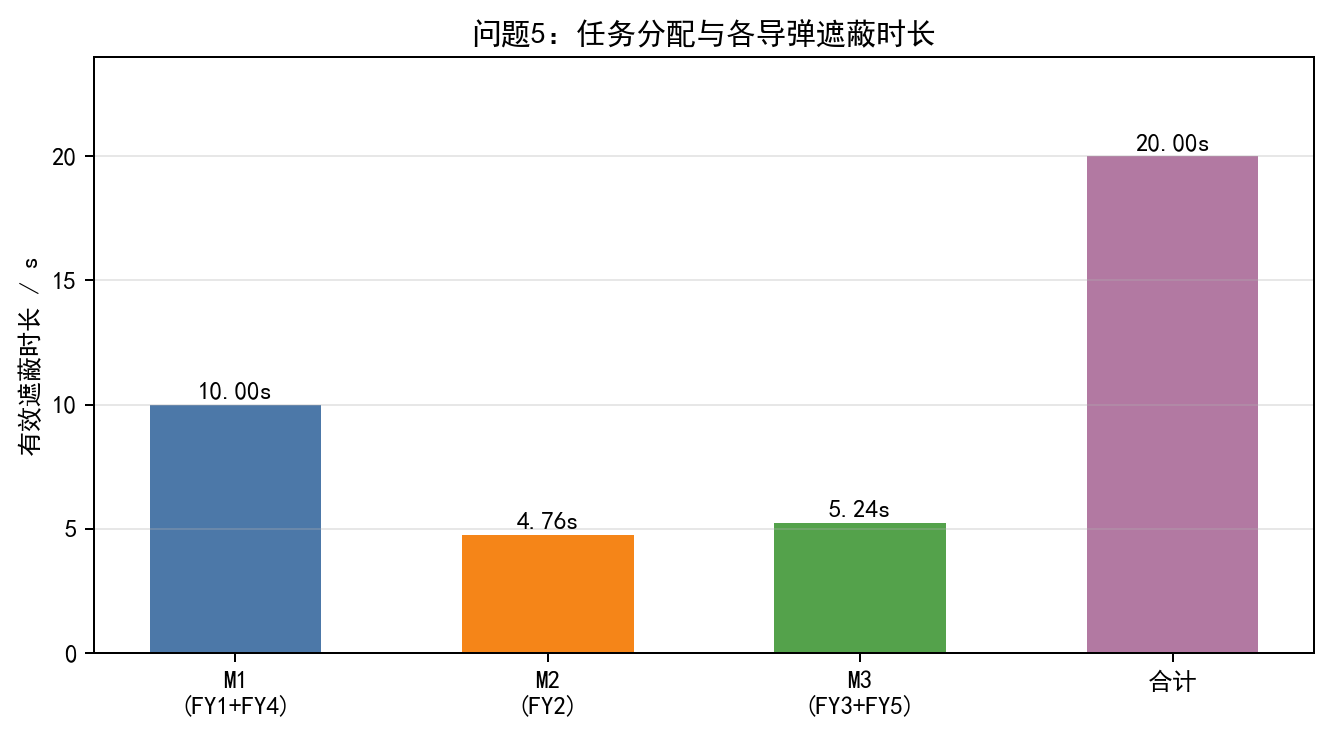
\includegraphics[width=0.72\textwidth]{q5_assignment_bar}
\caption{问题5：任务分配与各导弹遮蔽时长}
\label{fig:q5-bar}
\end{figure}

\begin{figure}[!htbp]
\centering
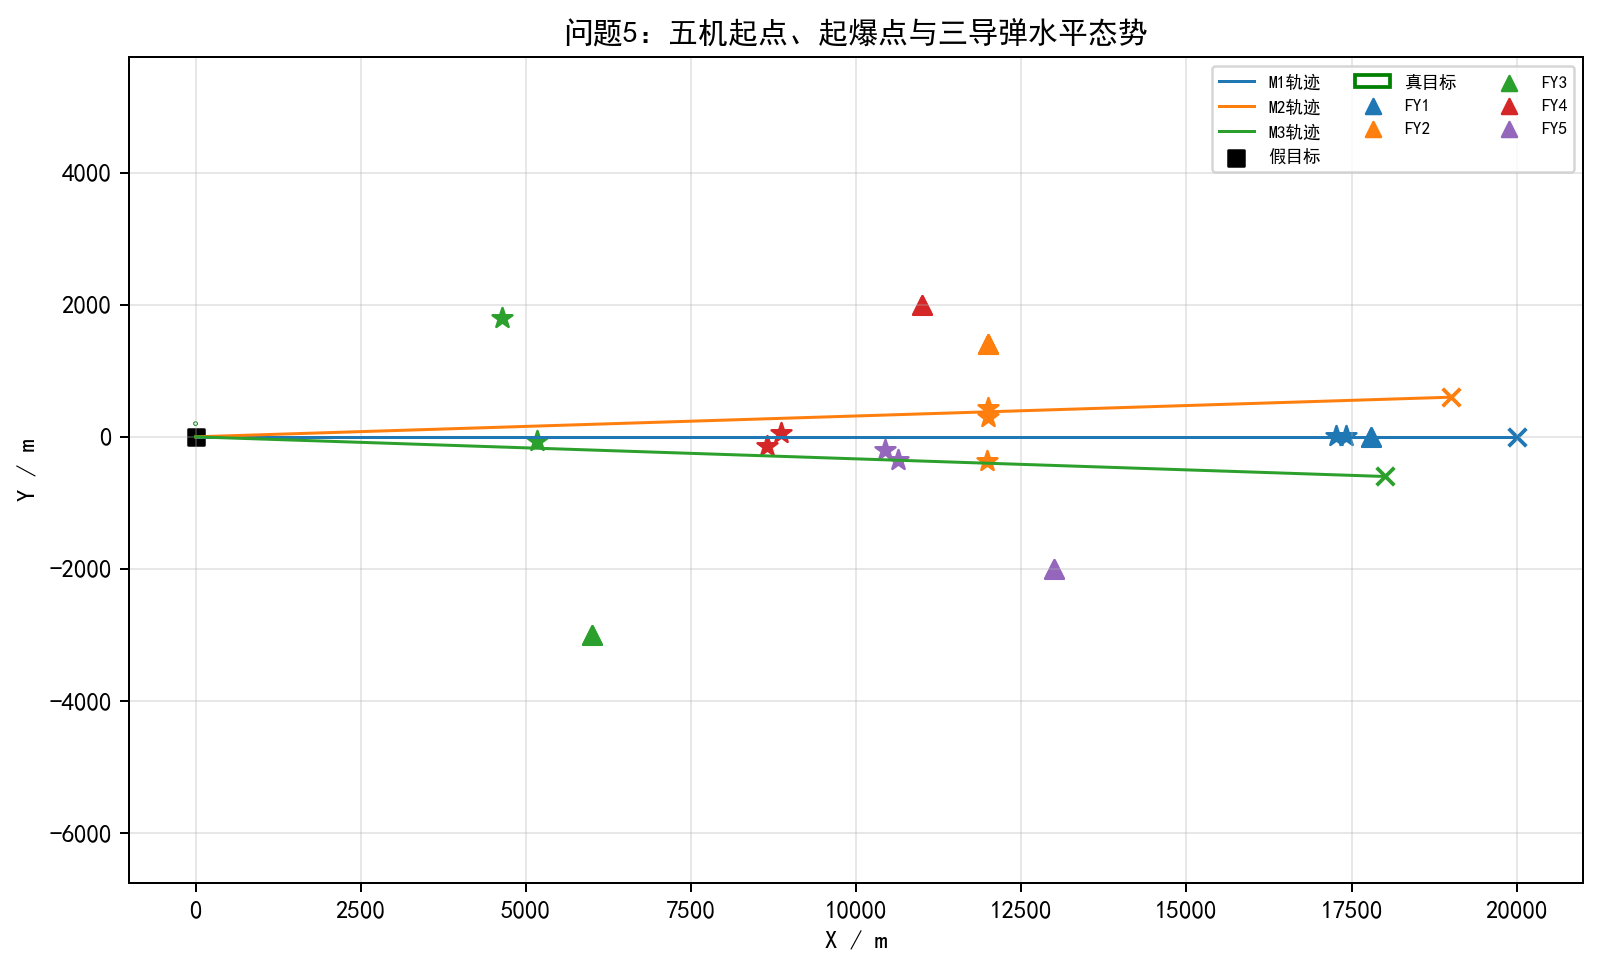
\includegraphics[width=0.82\textwidth]{q5_topview}
\caption{问题5：五机起点、起爆点与三导弹水平态势}
\label{fig:q5-top}
\end{figure}

\begin{figure}[!htbp]
\centering
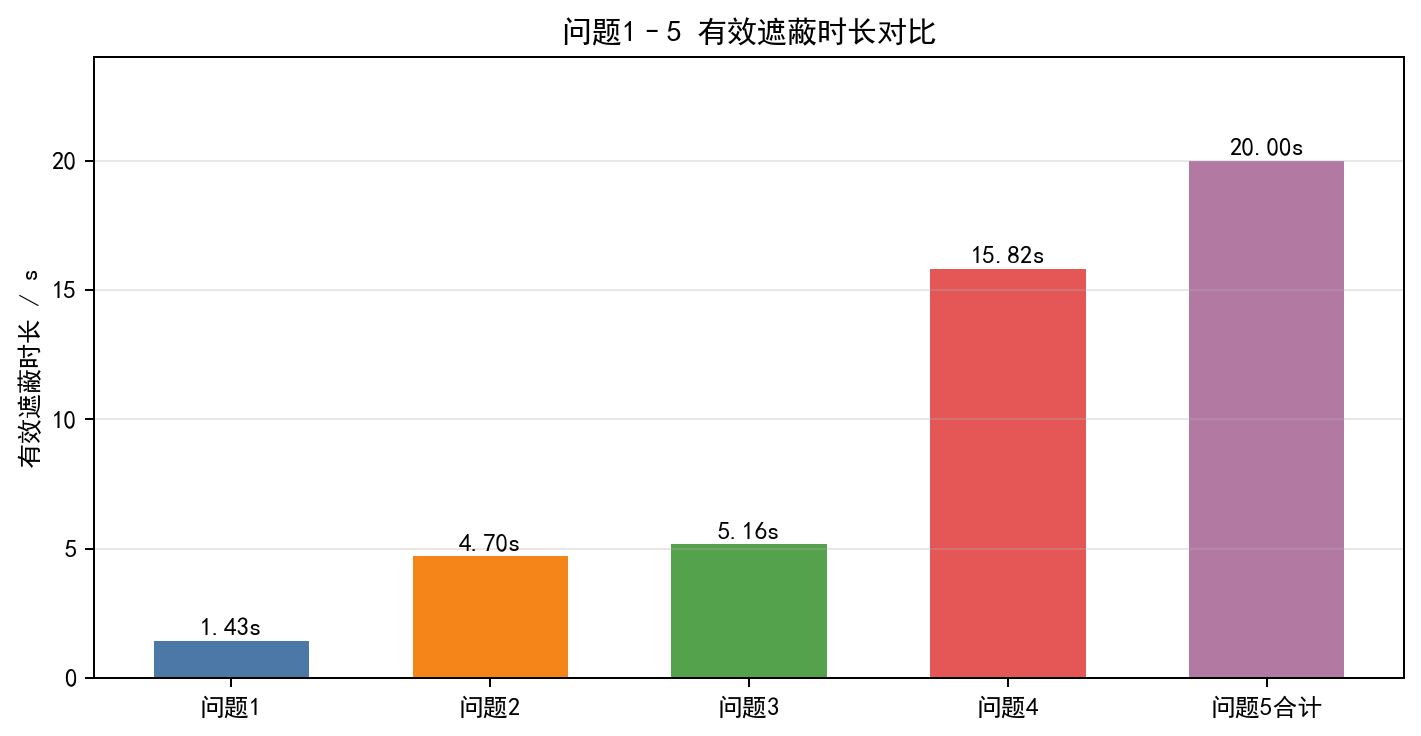
\includegraphics[width=0.78\textwidth]{q1_to_q5_duration_compare}
\caption{问题1–5 有效遮蔽时长对比}
\label{fig:all-cmp}
\end{figure}

\subsection{结果分析与讨论}
\begin{enumerate}
  \item \textbf{分层策略有效}：先分配后优化，使 5 机 11 弹的高维问题可在个人计算机上求解；
  \item \textbf{M1 获最长覆盖}：双机四弹前后接力，$J^{(M1)}=10\,\mathrm{s}$，显著高于单机单弹水平；
  \item \textbf{侧向导弹仍可覆盖}：尽管 M2/M3 初始方位偏移，FY2 与 FY3/FY5 仍分别贡献约 $4.8\,\mathrm{s}$ 与 $5.2\,\mathrm{s}$；
  \item \textbf{资源权衡}：若把更多弹集中给 M1，可能进一步提高 $J^{(M1)}$，但会削弱对 M2/M3 的保护；和式指标在“重点防护”与“全面覆盖”之间取得平衡。
\end{enumerate}

\section{模型评价与推广}

\subsection{优点}
\begin{enumerate}
  \item 运动学方程封闭、参数明确，便于复现与检验；
  \item 遮蔽判据几何意义清晰，把物理问题转化为可计算的距离条件；
  \item 决策变量参数化与动力学一致，避免“先给落点再反推”的不可行风险；
  \item 直接搜索对目标非光滑性不敏感，适合本问题。
\end{enumerate}

\subsection{不足与改进}
\begin{enumerate}
  \item 中心视线判据弱于“圆柱全表面视线均被遮挡”的严格判据，所得 $J$ 可能略偏乐观；后续可用柱面采样点做更严格检验；
  \item 网格搜索得到的是优良可行解，非严格全局最优，可进一步结合差分进化、贝叶斯优化等；
  \item 未计入风场、云团扩散、能见度阈值随时间衰减及导弹机动等因素。
\end{enumerate}

\subsection{推广}
问题3–5已将单弹模型扩展为多弹并集与多机分层优化。若进一步引入风场、云团扩散或导弹机动，可在同一遮蔽判据框架下替换运动学模块，而不改变优化分层结构。

\section{结论}
本文从“时变视线遮挡”出发，建立了烟幕干扰弹投放的运动学与几何判定模型，并完成五问求解。数值结果汇总如下：问题~1 给定策略下 $J_1=1.43\,\mathrm{s}$；问题~2 单弹优化后 $J_2=4.71\,\mathrm{s}$；问题~3 同机三弹并集 $J_3=5.16\,\mathrm{s}$；问题~4 三机协同 $J_4=15.82\,\mathrm{s}$；问题~5 五机对三导弹合计 $J_5=20.00\,\mathrm{s}$（M1/M2/M3 分别为 $10.00/4.76/5.24\,\mathrm{s}$）。比较可见：单机增弹的收益受共线航迹限制，而多机在不同空域错峰布置可近似实现窗口拼接，是延长有效遮蔽的主要途径。完整计算过程见笔记本 \texttt{A题\_烟幕干扰弹投放策略.ipynb}，策略表见 \texttt{result1.xlsx}--\texttt{result3.xlsx}。

\begin{thebibliography}{9}
\bibitem{cumcm2025}
全国大学生数学建模竞赛组委会.
\newblock 2025 年高教社杯全国大学生数学建模竞赛题目 A 题：烟幕干扰弹的投放策略.
\bibitem{format2023}
全国大学生数学建模竞赛组委会.
\newblock 全国大学生数学建模竞赛论文格式规范（2023 年修改）.
\bibitem{liuhaiyang2013latex}
刘海洋.
\newblock \LaTeX{}入门[M].
\newblock 北京：电子工业出版社, 2013.
\end{thebibliography}

\newpage
\begin{appendices}
\section{核心算法说明}
本文数值计算流程如下：
\begin{enumerate}
  \item 由决策变量计算投放点、起爆点与云团中心轨迹；
  \item 在有效时间窗上按步长 $\Delta t$ 离散，逐时刻计算点到线段距离；
  \item 单弹累计 $d(t)\le 10$ 的时长；多弹则对 $\min_i d_i(t)$ 做并集累计；
  \item 问题2--3：视线落点构造 + 网格/邻域搜索；问题4：分机优化后联合微调；问题5：任务分配后分层求解。
\end{enumerate}
完整程序文件：
\begin{itemize}
  \item \texttt{code/solve\_all\_problems.py}：问题1--5完整求解与结果导出（附录 B）；
  \item \texttt{code/gen\_q345\_figures.py}：问题3--5补充作图（附录 C）；
  \item \texttt{A题\_烟幕干扰弹投放策略.ipynb}：交互式复现笔记本；
  \item \texttt{result1.xlsx}--\texttt{result3.xlsx}：题目要求的结果表。
\end{itemize}

\lstset{
  language=Python,
  basicstyle=\ttfamily\zihao{-5},
  breaklines=true,
  columns=fullflexible,
  frame=single,
  numbers=left,
  numberstyle=\tiny,
  showstringspaces=false,
  tabsize=4,
  captionpos=b
}

\section{问题1--5完整 Python 源程序}
\label{app:code-all}
下列程序整合公共运动学/遮蔽判定模块与问题1--5求解、Excel导出及主要作图，可在项目根目录直接运行：
\begin{center}
\texttt{python code/solve\_all\_problems.py}
\end{center}

\lstinputlisting[caption={问题1--5完整求解程序（solve\_all\_problems.py）}]{code/solve_all_problems.py}

\section{问题3--5补充作图程序}
\label{app:code-fig}
下列程序根据 \texttt{result1.xlsx}--\texttt{result3.xlsx} 生成论文中问题3--5的补充图表：
\begin{center}
\texttt{python code/gen\_q345\_figures.py}
\end{center}

\lstinputlisting[caption={问题3--5补充作图程序（gen\_q345\_figures.py）}]{code/gen_q345_figures.py}

\end{appendices}

\end{document}
